\documentclass[10pt]{article}

%% Various useful packages and commands from different sources

\usepackage[applemac]{inputenc}
\usepackage[english]{babel}
\usepackage[T1]{fontenc}
\usepackage{cite, url,color} % Citation numbers being automatically sorted and properly "compressed/ranged".
%\usepackage{pgfplots}
\usepackage{graphics,amsfonts}
\usepackage[pdftex]{graphicx}
\usepackage[cmex10]{amsmath}
\usepackage{amssymb}
\usepackage{bm}
% Also, note that the amsmath package sets \interdisplaylinepenalty to 10000
% thus preventing page breaks from occurring within multiline equations. Use:
 \interdisplaylinepenalty=2500
% after loading amsmath to restore such page breaks as IEEEtran.cls normally does.

% Compact lists
\usepackage{enumitem}
\usepackage{booktabs}
\usepackage{fancyvrb}

% Tikz
\usepackage{tikz}
\usetikzlibrary{automata,positioning,chains,shapes,arrows}
\usepackage{pgfplots}
\usetikzlibrary{plotmarks}
\newlength\fheight
\newlength\fwidth
\pgfplotsset{compat=newest}
\pgfplotsset{plot coordinates/math parser=false}

\usepackage{listings} % for Matlab code
\definecolor{commenti}{rgb}{0.13,0.55,0.13}
\definecolor{stringhe}{rgb}{0.63,0.125,0.94}
\lstloadlanguages{Matlab}
\lstset{% general command to set parameter(s)
framexleftmargin=0mm,
frame=single,
keywordstyle = \color{blue},% blue keywords
identifierstyle =, % nothing happens
commentstyle = \color{commenti}, % comments
stringstyle = \ttfamily \color{stringhe}, % typewriter type for strings
showstringspaces = false, % no special string spaces
emph = {for, if, then, else, end},
emphstyle = \color{blue},
firstnumber = 1,
numbers =right, %  show number_line
numberstyle = \tiny, % style of number_line
stepnumber = 5, % one number_line after stepnumber
numbersep = 5pt,
language = {Matlab},
extendedchars = true,
breaklines = true,
breakautoindent = true,
breakindent = 30pt,
basicstyle=\footnotesize\ttfamily
}

\usepackage{array}
% http://www.ctan.org/tex-archive/macros/latex/required/tools/
\usepackage{mdwmath}
\usepackage{mdwtab}
%mdwtab.sty	-- A complete ground-up rewrite of LaTeX's `tabular' and  `array' environments.  Has lots of advantages over
%		   the standard version, and over the version in `array.sty'.
% *** SUBFIGURE PACKAGES ***
% \usepackage[tight,footnotesize]{subfigure}
\usepackage{subfig}
\usepackage[top=2.2cm, bottom=2.2cm, right=1.7cm,left=1.7cm]{geometry}
\usepackage{indentfirst}


%\setlength\parindent{0pt}
\linespread{1}

\usepackage{mathtools}
\DeclarePairedDelimiter{\ceil}{\lceil}{\rceil}
\DeclarePairedDelimiter{\floor}{\lfloor}{\rfloor}
\DeclareMathOperator*{\argmax}{arg\,max}
\DeclareMathOperator*{\argmin}{arg\,min}
\newcommand{\M} {\mathtt{M}}
\newcommand{\dB} {\mathrm{dB}}
\newcommand{\tr} {\mathrm{tr}}
\newcommand{\lmod}[1] {_{\,\mathrm{mod}\,#1}}
\newcommand{\outf}[1] {\mathcal{O}(#1)}
\newcommand{\SU}[1] {\mathcal{S}(#1)}
\newcommand{\s} {\mathbf{s}}
\newcommand{\y} {\mathbf{y}}


\graphicspath{ {figures/} }
\setcounter{MaxMatrixCols}{20}

% equations are numbered section by section
%\numberwithin{equation}{section}


\begin{document}
\title{Channel Coding 15/16 - Homework 2}
\author{Michele Polese}

\maketitle

% For tikz
% Definition of blocks:
\tikzstyle{block} = [draw, rectangle, 
    minimum height=1em, minimum width=1em]
\tikzstyle{circlenode} = [draw, circle, minimum height=3em, minimum width=3em]
\tikzstyle{trellisnode} = [draw, circle, minimum height=2em, minimum width=2em]
\tikzstyle{sum} = [draw, circle, node distance=1cm]
\tikzstyle{input} = [coordinate]
\tikzstyle{output} = [coordinate]
\tikzstyle{pinstyle} = [pin edge={to-,thin,black}]

In this report the solution to Exercises 4, 9 and 11 will be discussed. In the attached file there is the code that was developed to solve these exercises.

%%%%%%%%%%%%%%%%%%%%%%%%%%%%%%%%%%%%%%%%%
%%%%%%%%%%%%%% PROBLEM 4 %%%%%%%%%%%%%%%%
%%%%%%%%%%%%%%%%%%%%%%%%%%%%%%%%%%%%%%%%%

\section*{Exercise 4 - Non linear encoding}
In this exercise we will analyze sum-product and min-sum algorithms applied to a non linear element in a code. As first we will discuss the factor graph, its behavioral function, then an approach for marginalization when a decision on input symbols has to be taken, and finally we will present more general results to be applied whenever the node is part of a more complex factor graph.

\subsection*{Non linear code}
Consider the non linear code that maps the binary sequence $u_0, u_1, u_2, \dots$ into $c_0, c_1, c_2, c_3, c_4, c_5, c_6, \dots$ by grouping input bits into pairs and applying the non linear relation of equation~\eqref{eq:nlmap}.

\begin{equation}\label{eq:nlmap}
\centering
	\begin{array} {ccccccc}
		u_0 & u_1 & \rightarrow & c_0 & c_1 & c_2 & c_3 \\
		0 & 0 & \rightarrow & 0 & 0 & 0 & 0 \\
		0 & 1 & \rightarrow & 1 & 0 & 0 & 0 \\
		1 & 0 & \rightarrow & 0 & 1 & 0 & 0 \\
		1 & 1 & \rightarrow & 0 & 0 & 1 & 0 \\
	\end{array}
\end{equation}

Assume that $u_i$ symbols are IID, that the transmission happens on an AWGN channel and that $c_i$ are mapped into transmitted symbols $s_i$ such that

\begin{equation}\label{eq:lmap}
	s_i = \mathcal{L}(c_i) =
	\begin{cases}
		+1 & \mbox{ if } c_i = 1 \\
		-1 & \mbox{ if } c_i = 0 \\
	\end{cases}
\end{equation}

The objective of this exercise is to find compact expressions for the LLR that can be used when applying sum-product or min-sum algorithms to decode a message encoded with~\eqref{eq:nlmap}.
Let's introduce the node $w$ as in Fig.~\ref{fig:factornode}.
\begin{figure}[h]
\centering
\begin{tikzpicture}[auto, thick, node distance=1 cm]
	\node[block] (w) {$w$};
	\node[left= 2cm of w] (place1) {};
	\node[below=0.3cm of place1] (c1) {};
	\node[below of=c1] (c0) {};
	\node[above of=c1] (c2) {};
	\node[above of=c2] (c3) {};
	\node[right= 2cm of w] (place2) {};
	\node[below= 0.75cm of place2] (u0) {};
	\node[above= 0.75cm of place2] (u1) {};

	\path[every node]
		(c3) edge node[below] {$c_3$} (w)
		(c2) edge node[below] {$c_2$} (w)
		(c1) edge node[below] {$c_1$} (w)
		(c0) edge node[below] {$c_0$} (w)
		(u0) edge node[below] {$u_0$} (w)
		(u1) edge node[below] {$u_1$} (w);
\end{tikzpicture}
\caption{Factor node $w$}
\label{fig:factornode}
\end{figure}

Let $w$ be the behavioral function for the transformation~\eqref{eq:nlmap}, so that
\begin{equation}\label{eq:beha}
	w(c_0, c_1, c_2, c_3, u_0, u_1) =
	\begin{cases}
		1 & \mbox{ if } c_0c_1c_2c_3 \mbox{ is the codeword associated with } u_0u_1 \\
		0 & \mbox{ otherwise}
	\end{cases}
\end{equation}

By using~\eqref{eq:beha} it is possible to express the MAP criterion to decide on $\hat{u}_i$ in a simple form

\begin{equation}
	\hat{u}_i = \argmax_{a} \sum_{\mathbf{c}} \sum_{\mathbf{u} \sim u_i} w(\mathbf{c}, \mathbf{u}) p(\boldsymbol{\rho}_m | \mathbf{c}) p(\mathbf{u}_m = \mathbf{u})
\end{equation}

In particular, given the fact that $u_i$ depends only on 4 $c_j$, i.e. for $j \in [2(i-\bmod(i,2)), 2(i-\bmod(i,2) + 1) - 1]$, it is possible to consider the pair $[u_i, u_{i+1}]_{\bmod(i,2) = 0}$ and the associated 4-tuple $[c_{2i}, c_{2i+1}, c_{2i+2}, c_{2i+3}]$. 
For simplicity from now on we will analyze MAP decoding for $[u_0, u_1]$ and associated codeword $[c_0, c_1, c_2, c_3]$. 

Then given independent input symbols the MAP criterion becomes
\begin{equation}\label{eq:u0}
	\hat{u}_0 = \argmax_{a \in [0,1]} \sum_{c_0, c_1, c_2, c_3} \sum_{u_1} w(c_0, c_1, c_2, c_3, u_0, u_1) p(\boldsymbol{\rho}_0 | c_0, c_1, c_2, c_3) p(u_0 = a) p(u_1)
\end{equation}

\begin{equation}\label{eq:u1}
	\hat{u}_1 = \argmax_{a \in [0,1]} \sum_{c_0, c_1, c_2, c_3} \sum_{u_0} w(c_0, c_1, c_2, c_3, u_0, u_1) p(\boldsymbol{\rho}_0 | c_0, c_1, c_2, c_3) p(u_0) p(u_1 = a) 
\end{equation}

Note that under the hypothesis of having an AWGN channel and given $\boldsymbol{\rho}_0 = [r_0, r_1, r_2, r_3]$ then
\begin{equation}
	p(\boldsymbol{\rho}_0 | c_0, c_1, c_2, c_3) = \Pi_{i = 0}^{3} g(r_i | c_i)
\end{equation}
with
\begin{equation}
	g(r_i|c_i) = \frac{1}{\sqrt{2\pi \sigma_w^2}} e^{-\frac{(r_i - \mathcal{L}(c_i))^2}{2\sigma_w^2}}
\end{equation}
Message passing can be used to solve~\eqref{eq:u0} and~\eqref{eq:u1}. In the particular define the APP (a posteriori probability) as the product
\begin{equation}\label{eq:APP}
	w(c_0, c_1, c_2, c_3, u_0, u_1) \Pi_{i = 0}^{3} g(r_i | c_i)p(u_0) p(u_1) 
\end{equation}
The APP can be represented by the Forney-style Factor Graph in Fig.~\ref{fig:FFG}.

\begin{figure}[h]
\centering
\begin{tikzpicture}[auto, thick, node distance=1 cm]
	\node[block] (w) {$w$};
	\node[left= 2cm of w] (place1) {};
	\node[block, below=0.1cm of place1] (c1) {$g(r_1|c_1)$};
	\node[block, below of=c1] (c0) {$g(r_0|c_0)$};
	\node[block, above of=c1] (c2) {$g(r_2|c_2)$};
	\node[block, above of=c2] (c3) {$g(r_3|c_3)$};
	\node[block, below right=1cm of w] (u0) {$p(u_0)$};
	\node[block, above right=1cm of w] (u1) {$p(u_1)$};

	\path[every node]
		(c3) edge node[above] {$c_3$} (w)
		(c2) edge node[above left] {$c_2$} (w)
		(c1) edge node[below left] {$c_1$} (w)
		(c0) edge node[below] {$c_0$} (w)
		(u0) edge node[below] {$u_0$} (w)
		(u1) edge node[above] {$u_1$} (w);
\end{tikzpicture}
\caption{FFG for the APP~\eqref{eq:APP}}
\label{fig:FFG}
\end{figure}

\subsection*{Sum-product algorithm}

Let's apply sum-product algorithm to the FFG in Fig.~\ref{fig:FFG}. Compute $\mu_{w\rightarrow u_0} (u_0)$ and then the LLR associated with this message.
Let $\mu_{c_i\rightarrow w}(c_i) = g(r_i|c_i)$ and $\mu_{u_i \rightarrow w}(u_i) = p(u_i)$. Then
\begin{equation}\label{eq:u0form1}
	\mu_{w\rightarrow u_0} (u_0) = \sum_{c_0, c_1, c_2, c_3, u_1} w(c_0, c_1, c_2, c_3, u_0, u_1) \Pi_{i=0}^{3}\mu_{c_i\rightarrow w} (c_i) \mu_{u_1 \rightarrow w} (u_1) 
\end{equation}
and
\begin{equation}
	LLR_{w\rightarrow u_0} = \ln \left( \frac{\mu_{w\rightarrow u_0} (0)}{\mu_{w\rightarrow u_0} (1)} \right)
\end{equation}
Because of the behavioral function $w$ the numerator has terms different from $0$ only for $u_1 = 0, c_i = 0 \; \forall i$ and $u_1 = c_0 = 1, c_1 = c_2 = c_3 = 0$. For the same reason at the denominator the non zero terms are for $u_1 = c_0 = c_2 = c_3 = 0, c_1 = 1$ and $u_1 = c_2 = 1, c_0 = c_1 = c_3 = 0$. In particular notice that $c_3 = 0$ in every case.
Then 
\begin{equation}
	LLR_{w\rightarrow u_0} = \ln 
		\left( 
		\frac{g(r_0|0)g(r_1|0)g(r_2|0)g(r_3|0)p(u_1=0) + g(r_0|1)g(r_1|0)g(r_2|0)g(r_3|0)p(u_1=1)}
		{g(r_0|0)g(r_1|1)g(r_2|0)g(r_3|0)p(u_1=0) + g(r_0|0)g(r_1|0)g(r_2|1)g(r_3|0)p(u_1=1)}
		\right)
\end{equation}
The factor $g(r_3|0)$ can be simplified, as like as the $(\frac{1}{\sqrt{2\pi \sigma_w^2}})^4$ which is given by the product of the channel transition probabilities. Then notice that
\begin{equation} \label{eq:power}
	e^{(r_i + 1)^2} + e^{(r_i - 1)^2} = 
	e^{r_i^2}e^{2r_i}e^{1} + e^{r_i^2}e^{-2r_1}e^{1} = e^{r_i^2 + 1} (e^{2r_i} + e^{-2r_1})
\end{equation} 
Equation~\eqref{eq:power} can be used to collect terms of $g(r_0|0)$ and $g(r_0|1)$ in the summation at the numerator, as well as $g(r_1|0)$, $g(r_1|1)$ and $g(r_2|0)$, $g(r_2|1)$ at the denominator. Then
\begin{equation}
	LLR_{w\rightarrow u_0} = \ln 
		\left( 
		\frac{
			e^{-\frac{1}{2\sigma_w^2} ((r_1+1)^2+(r_2+1)^2+r_0^2+1)}
				\left[
					e^{-\frac{2r_0}{2\sigma_w^2}}p(u_1=0)+e^{-\frac{-2r_0}{2\sigma_w^2}}p(u_1=1)
				\right]
		}{
			e^{-\frac{1}{2\sigma_w^2} ((r_0+1)^2+r_1^2+1+r_2^2+1)}
				\left[
					e^{-\frac{-2r_1 + 2r_2}{2\sigma_w^2}}p(u_1=0)+e^{-\frac{2r_1 - 2r_2}{2\sigma_w^2}}p(u_1=1)
				\right]
		}
		\right)
\end{equation}

\begin{equation}
	LLR_{w\rightarrow u_0} = \ln 
		\left( 
		\frac{
			e^{-\frac{2r_1+2r_2}{2\sigma_w^2}}
				\left[
					e^{-\frac{2r_0}{2\sigma_w^2}}p(u_1=0)+e^{-\frac{-2r_0}{2\sigma_w^2}}p(u_1=1)
				\right]
		}{
			e^{-\frac{2r_0}{2\sigma_w^2}}
				\left[
					e^{-\frac{-2r_1 + 2r_2}{2\sigma_w^2}}p(u_1=0)+e^{-\frac{2r_1 - 2r_2}{2\sigma_w^2}}p(u_1=1)
				\right]
		}
		\right)
\end{equation}


\begin{equation}
	LLR_{w\rightarrow u_0} = 
	\frac{1}{\sigma_w^2}(r_0 - r_1 - r_2) + 
	\ln 
		\left( 
		\frac{
			e^{-\frac{r_0}{\sigma_w^2}}p(u_1=0)+e^{\frac{r_0}{\sigma_w^2}}p(u_1=1)
		}{
			e^{\frac{r_1 - r_2}{\sigma_w^2}}p(u_1=0)+e^{-\frac{r_1 - r_2}{\sigma_w^2}}p(u_1=1)
		}
		\right)
\end{equation}
and in the case in which $p(u_1 = 0) = p(u_1 = 1)$ this expression becomes
\begin{equation}\label{eq:llru0final}
	LLR_{w\rightarrow u_0} = 
	\frac{1}{\sigma_w^2}(r_0 - r_1 - r_2) + 
	\ln 
		\left( 
		\frac{
			\cosh{\frac{r_0}{\sigma_w^2}}
		}{
			\cosh{\frac{r_1-r_2}{\sigma_w^2}}
		}
		\right)
\end{equation}
The same computation can be carried out for $\mu_{w\rightarrow u_1} (u_1)$:
\begin{equation}
	\mu_{w\rightarrow u_1} (u_1) = \sum_{c_0, c_1, c_2, c_3, u_0} w(c_0, c_1, c_2, c_3, u_0, u_1) \Pi_{i=0}^{3}\mu_{c_i\rightarrow w} (c_i) \mu_{u_0 \rightarrow w} (u_0) 
\end{equation}
and 
\begin{equation}
	LLR_{w\rightarrow u_1} = \ln \left( \frac{\mu_{w\rightarrow u_1} (0)}{\mu_{w\rightarrow u_1} (1)} \right)
\end{equation}
The numerator has terms different from zero in the summation only for $u_0 = c_i = 0, \forall i$ and $u_0 = c_1 = 1, c_0 = c_2 = c_3 = 0$ and the denominator for $u_0 = c_1 = c_2 = c_3 = 0, c_0 = 1$ and $u_0 = c_2 = 1, c_0 = c_1 = c_3 = 0$, so that
\begin{equation}
	LLR_{w\rightarrow u_1} = \ln 
		\left( 
		\frac{g(r_0|0)g(r_1|0)g(r_2|0)g(r_3|0)p(u_0=0) + g(r_0|0)g(r_1|1)g(r_2|0)g(r_3|0)p(u_0=1)}
		{g(r_0|1)g(r_1|0)g(r_2|0)g(r_3|0)p(u_0=0) + g(r_0|0)g(r_1|0)g(r_2|1)g(r_3|0)p(u_0=1)}
		\right)
\end{equation}
Note that once again $g(r_3|0)$ can be simplified, as like as $(\frac{1}{\sqrt{2\pi \sigma_w^2}})^4$. Then by using~\eqref{eq:power} the LLR can be simplified to

\begin{equation}
	LLR_{w\rightarrow u_1} = \ln 
		\left( 
		\frac{
			e^{-\frac{1}{2\sigma_w^2} ((r_0+1)^2+(r_2+1)^2+r_1^2+1)}
				\left[
					e^{-\frac{2r_1}{2\sigma_w^2}}p(u_0=0)+e^{-\frac{-2r_1}{2\sigma_w^2}}p(u_0=1)
				\right]
		}{
			e^{-\frac{1}{2\sigma_w^2} ((r_1+1)^2+r_0^2+1+r_2^2+1)}
				\left[
					e^{-\frac{-2r_0 + 2r_2}{2\sigma_w^2}}p(u_0=0)+e^{-\frac{2r_0 - 2r_2}{2\sigma_w^2}}p(u_0=1)
				\right]
		}
		\right)
\end{equation}

\begin{equation}
	LLR_{w\rightarrow u_1} = \ln 
		\left( 
		\frac{
			e^{-\frac{2r_0+2r_2}{2\sigma_w^2}}
				\left[
					e^{-\frac{2r_1}{2\sigma_w^2}}p(u_0=0)+e^{-\frac{-2r_0}{2\sigma_w^2}}p(u_0=1)
				\right]
		}{
			e^{-\frac{2r_1}{2\sigma_w^2}}
				\left[
					e^{-\frac{-2r_0 + 2r_2}{2\sigma_w^2}}p(u_0=0)+e^{-\frac{2r_0 - 2r_2}{2\sigma_w^2}}p(u_0=1)
				\right]
		}
		\right)
\end{equation}

\begin{equation}
	LLR_{w\rightarrow u_1} = 
	\frac{1}{\sigma_w^2}(r_1 - r_0 - r_2) + 
	\ln 
		\left( 
		\frac{
			e^{-\frac{r_1}{\sigma_w^2}}p(u_0=0)+e^{\frac{r_1}{\sigma_w^2}}p(u_0=1)
		}{
			e^{\frac{r_0 - r_2}{\sigma_w^2}}p(u_0=0)+e^{-\frac{r_0 - r_2}{\sigma_w^2}}p(u_0=1)
		}
		\right)
\end{equation}
and in the case in which $p(u_0 = 0) = p(u_0 = 1)$ this expression becomes
\begin{equation}\label{eq:llru1final}
	LLR_{w\rightarrow u_1} = 
	\frac{1}{\sigma_w^2}(r_1 - r_0 - r_2) + 
	\ln 
		\left( 
		\frac{
			\cosh{\frac{r_1}{\sigma_w^2}}
		}{
			\cosh{\frac{r_0-r_2}{\sigma_w^2}}
		}
		\right)
\end{equation}
It can be seen that $LLR_{w\rightarrow u_0}$ and $LLR_{w\rightarrow u_1}$ share a similar structure.
Eventually it is possible to carry out a marginalization and a decision on $u_i$, i.e.
\begin{equation}
\hat{u}_i = \begin{cases}
				0 & \mbox{ if } LLR_{w\rightarrow u_i} + LLR_{p\rightarrow u_i} \ge 0 \\
				1 & \mbox{ otherwise } \\
			\end{cases}
\end{equation}
with
\begin{equation}
LLR_{p\rightarrow u_i} = \ln \left( \frac{p(u_i = 0)}{p(u_i=1)} \right)
\end{equation}

\subsection*{Min-sum algorithm}
Let's consider also the min-sum algorithm and define the messages exiting from leafs as
\begin{equation}
	\hat{\mu}_{c_i \rightarrow w}(c_i) = -\ln(g(r_i|c_i)) = -\ln\left(\frac{1}{\sqrt{2\pi \sigma_w^2}} e^{-\frac{(r_i - \mathcal{L}(c_i))^2}{2\sigma_w^2}}\right) = \frac{1}{2\sigma_w^2}(r_i - \mathcal{L}(c_i))^2 - \ln\left(\frac{1}{\sqrt{2\pi \sigma_w^2}}\right)
\end{equation}
and
\begin{equation}
	\hat{\mu}_{u_i \rightarrow w}(u_i) = -\ln(p(u_i)) := \hat{p}(u_i) 
\end{equation}
Let $\alpha = - \ln\left(\frac{1}{\sqrt{2\pi \sigma_w^2}}\right)$ be a constant which will be simplified in the LLR. Then by applying min-sum to the message from $w$ to $u_0$ we have
\begin{equation}\label{eq:minsum}
	\hat{\mu}_{w \rightarrow u_0}(u_0) = \min_{c_0, c_1, c_2, c_3, u_1} 
		\left\{
			-\ln(w(c_0, c_1, c_2, c_3, u_0, u_1)) + 
			\sum_{i=0}^{3} \hat{\mu}_{c_i \rightarrow w}(c_i) + \hat{\mu}_{u_1 \rightarrow w}(u_1)
		\right\}
\end{equation}
Notice that if $w(c_0, c_1, c_2, c_3, u_0, u_1) = 0$ then $-\ln(w(c_0, c_1, c_2, c_3, u_0, u_1)) = \infty$, i.e. if a combination $(c_0, c_1, c_2, c_3, u_0, u_1)$ is not a valid coded/uncoded couple then it will not be surely chosen as the one that yields the minimum value in~\eqref{eq:minsum}. Therefore~\eqref{eq:minsum} can be written as
\begin{equation}\label{eq:minsum2}
	\hat{\mu}_{w \rightarrow u_0}(u_0) = \min_{c_0, c_1, c_2, c_3, u_1 | w(c_0, c_1, c_2, c_3, u_0, u_1) = 1} 
		\left\{
			\sum_{i=0}^{3} \hat{\mu}_{c_i \rightarrow w}(c_i) + \hat{\mu}_{u_1 \rightarrow w}(u_1)
		\right\}
\end{equation}
Then the LLR can be computed as
\begin{equation}
	LLR_{w \rightarrow u_0} = \hat{\mu}_{w \rightarrow u_0}(1) - \hat{\mu}_{w \rightarrow u_0}(0)
\end{equation}

\begin{multline}\label{eq:LLR1}
	LLR_{w \rightarrow u_0} = 
	\min_{c_0, c_1, c_2, c_3, u_1 | w(c_0, c_1, c_2, c_3, 1, u_1) = 1} 
		\left\{
			\sum_{i=0}^{3} \hat{\mu}_{c_i \rightarrow w}(c_i) + \hat{\mu}_{u_1 \rightarrow w}(u_1)
		\right\}
	- \\
	\min_{c_0, c_1, c_2, c_3, u_1 | w(c_0, c_1, c_2, c_3, 0, u_1) = 1} 
		\left\{
			\sum_{i=0}^{3} \hat{\mu}_{c_i \rightarrow w}(c_i) + \hat{\mu}_{u_1 \rightarrow w}(u_1)
		\right\} = \\
	\min
		\bigg\{
			\frac{1}{2\sigma_w^2}\left[(r_0+1)^2 + (r_1-1)^2 + (r_2+1)^2 + (r_3+1)^2\right] + 4\alpha + \hat{p}(u_1 = 0), \\
			\frac{1}{2\sigma_w^2}\left[(r_0+1)^2 + (r_1+1)^2 + (r_2-1)^2 + (r_3+1)^2\right] + 4\alpha + \hat{p}(u_1 = 1)
		\bigg\} \\
	 - \min
		\bigg\{
			\frac{1}{2\sigma_w^2}\left[(r_0+1)^2 + (r_1+1)^2 + (r_2+1)^2 + (r_3+1)^2\right] + 4\alpha + \hat{p}(u_1 = 0), \\
			\frac{1}{2\sigma_w^2}\left[(r_0-1)^2 + (r_1+1)^2 + (r_2+1)^2 + (r_3+1)^2\right] + 4\alpha + \hat{p}(u_1 = 1)
		\bigg\}
\end{multline}
Note that also for the min-sum LLRs it is possible to exploit a relation similar to~\eqref{eq:power}, i.e.
\begin{equation}
	\min\{a+b+c, a+b+d\} = a+b+\min\{c,d\}
\end{equation}
Then $4\alpha$ and $(r_3+1)^2$ can be simplified and~\eqref{eq:LLR1} becomes
\begin{multline}\label{eq:LLR1semifinal}
	LLR_{w \rightarrow u_0} = \frac{1}{2\sigma_w^2}\left[ (r_0+1)^2 + r_1^2 + 1 + r_2^2+1 \right] + \min\left\{ \frac{1}{2\sigma_w^2}(-2r_1 + 2r_2) + \hat{p}(u_1=0), \frac{1}{2\sigma_w^2}(2r_1 - 2r_2) + \hat{p}(u_1=1) \right\} \\
	- \frac{1}{2\sigma_w^2}\left[ (r_1+1)^2 + (r_2+1)^2 +r_0^2 + 1 \right] -
	\min\left\{ \frac{1}{2\sigma_w^2}(2r_0) + \hat{p}(u_1=0), \frac{1}{2\sigma_w^2}(- 2r_0) + \hat{p}(u_1=1) \right\} = \\
	\frac{1}{\sigma_w^2}\left[r_0 - r_1 - r_2 \right] + \min\left\{ \frac{r_2-r_1}{\sigma_w^2} + \hat{p}(u_1=0), \frac{r_1-r_2}{\sigma_w^2} + \hat{p}(u_1=1) \right\} \\ -
	\min\left\{ \frac{r_0}{\sigma_w^2} + \hat{p}(u_1=0), \frac{-r_0}{\sigma_w^2} + \hat{p}(u_1=1) \right\}
\end{multline}
Eventually in case of equally likely input symbols~\eqref{eq:LLR1semifinal} becomes
\begin{equation}\label{eq:llrmin0}
	LLR_{w \rightarrow u_0} = \frac{1}{\sigma_w^2}\left\{ r_0 - r_1 - r_2 + |r_0| - |r_2 - r_1| \right\}
\end{equation}
by observing that 
\begin{equation}
	\min\{x, -x\} = 
	\begin{cases}
		-x & \mbox{ if } x \ge 0 \\
		x & \mbox{ if } x < 0
	\end{cases} = 
	- |x|
\end{equation}
The same computation can be carried out for 
\begin{equation}
	\hat{\mu}_{w \rightarrow u_1}(u_1) = \min_{c_0, c_1, c_2, c_3, u_0 | w(c_0, c_1, c_2, c_3, u_0, u_1) = 1} 
		\left\{
			\sum_{i=0}^{3} \hat{\mu}_{c_i \rightarrow w}(c_i) + \hat{\mu}_{u_0 \rightarrow w}(u_0)
		\right\}
\end{equation}
Once again the LLR can be computed as
\begin{equation}
	LLR_{w \rightarrow u_1} = \hat{\mu}_{w \rightarrow u_1}(1) - \hat{\mu}_{w \rightarrow u_1}(0)
\end{equation}
\begin{multline}\label{eq:LLR2}
	LLR_{w \rightarrow u_1} = 
	\min_{c_0, c_1, c_2, c_3, u_0 | w(c_0, c_1, c_2, c_3, u_0, 1) = 1} 
		\left\{
			\sum_{i=0}^{3} \hat{\mu}_{c_i \rightarrow w}(c_i) + \hat{\mu}_{u_0 \rightarrow w}(u_0)
		\right\}
	- \\
	\min_{c_0, c_1, c_2, c_3, u_0 | w(c_0, c_1, c_2, c_3, u_0, 0) = 1}  
		\left\{
			\sum_{i=0}^{3} \hat{\mu}_{c_i \rightarrow w}(c_i) + \hat{\mu}_{u_0 \rightarrow w}(u_0)
		\right\} = \\
	 = \min
		\bigg\{
			\frac{1}{2\sigma_w^2}\left[(r_0-1)^2 + (r_1+1)^2 + (r_2+1)^2 + (r_3+1)^2\right] + 4\alpha + \hat{p}(u_0 = 0), \\
			\frac{1}{2\sigma_w^2}\left[(r_0+1)^2 + (r_1+1)^2 + (r_2-1)^2 + (r_3+1)^2\right] + 4\alpha + \hat{p}(u_0 = 1)
		\bigg\} \\
	 - \min
		\bigg\{
			\frac{1}{2\sigma_w^2}\left[(r_0+1)^2 + (r_1+1)^2 + (r_2+1)^2 + (r_3+1)^2\right] + 4\alpha + \hat{p}(u_0 = 0), \\
			\frac{1}{2\sigma_w^2}\left[(r_0+1)^2 + (r_1-1)^2 + (r_2+1)^2 + (r_3+1)^2\right] + 4\alpha + \hat{p}(u_0 = 1)
		\bigg\} = \\
	 = \frac{1}{2\sigma_w^2}\left[ (r_1+1)^2 + r_0^2 + 1 + r_2^2+1 \right] + \min\left\{ \frac{1}{2\sigma_w^2}(-2r_0 + 2r_2) + \hat{p}(u_0=0), \frac{1}{2\sigma_w^2}(2r_0 - 2r_2) + \hat{p}(u_0=1) \right\} \\
	- \frac{1}{2\sigma_w^2}\left[ (r_0+1)^2 + (r_2+1)^2 +r_1^2 + 1 \right] - \min\left\{ \frac{1}{2\sigma_w^2}(2r_1) + \hat{p}(u_0=0), \frac{1}{2\sigma_w^2}(- 2r_1) + \hat{p}(u_0=1) \right\}
\end{multline}
and eventually
\begin{multline}
LLR_{w \rightarrow u_1} = 
		\frac{1}{\sigma_w^2}\left[r_1 - r_0 - r_2 \right] + \min\left\{ \frac{r_2-r_0}{\sigma_w^2} + \hat{p}(u_0=0), \frac{r_0-r_2}{\sigma_w^2} + \hat{p}(u_0=1) \right\} \\ -
		\min\left\{ \frac{r_1}{\sigma_w^2} + \hat{p}(u_0=0), \frac{-r_1}{\sigma_w^2} + \hat{p}(u_0=1) \right\}
\end{multline}
which in case of equally likely input symbols becomes
\begin{equation}\label{eq:llrmin1}
	LLR_{w \rightarrow u_1} = \frac{1}{\sigma_w^2}\left\{ r_1 - r_0 - r_2 + |r_1| - |r_2 - r_0| \right\}
\end{equation}

Finally the decision rule on $u_i$ is
\begin{equation}
\hat{u}_i = \begin{cases}
				0 & \mbox{ if } LLR_{w\rightarrow u_i} + LLR_{p\rightarrow u_i} \ge 0 \\
				1 & \mbox{ otherwise } \\
			\end{cases}
\end{equation}
with
\begin{equation}
LLR_{p\rightarrow u_i} = \ln \left( \frac{p(u_i = 0)}{p(u_i=1)} \right) = \hat{p}(u_i = 1) - \hat{p}(u_i = 0)
\end{equation}

\subsection*{Sum-product and min-sum with LLRs}
Let's consider the case in which the node in Fig.~\ref{fig:factornode} is part of a more complex factor graph, i.e. the case in which the messages $\mu_{c_i \rightarrow w}$ are not necessarily given by $g(r_i|c_i)$ and $\mu_{u_i \rightarrow w}$ by $p(u_i)$. Let's consider generically their LLR and remark that
\begin{equation}
	\mu(0) = \frac{e^{LLR}}{1+e^{LLR}}, \quad \quad \mu(1) = \frac{1}{1+e^{LLR}}
\end{equation}
Then~\eqref{eq:u0form1} becomes
\begin{equation}
	\mu_{w\rightarrow u_0} (u_0) = \sum_{c_0, c_1, c_2, c_3, u_1} w(c_0, c_1, c_2, c_3, u_0, u_1) \Pi_{i=0}^{3} \frac{e^{(1\oplus c_i)LLR_{c_i\rightarrow w}}}{1+e^{LLR_{c_i\rightarrow w}}} \frac{e^{(1\oplus u_1)LLR_{u_1\rightarrow w}}}{1+e^{LLR_{u_1\rightarrow w}}}
\end{equation}
The LLR is derived as follows, by reporting just the terms of the summation which are different from 0 and simplifying the common denominator given by the $1+e^{LLR_i}$ terms.
\begin{multline}
	LLR_{w\rightarrow u_0} = \ln \left(
				\frac{e^{LLR_{c_0 \rightarrow w}}e^{LLR_{c_1 \rightarrow w}}e^{LLR_{c_2 \rightarrow w}}e^{LLR_{c_3 \rightarrow w}}e^{LLR_{u_1 \rightarrow w}} + e^{LLR_{c_1 \rightarrow w}}e^{LLR_{c_2 \rightarrow w}}e^{LLR_{c_3 \rightarrow w}}}
				{e^{LLR_{c_0 \rightarrow w}}e^{LLR_{c_2 \rightarrow w}}e^{LLR_{c_3 \rightarrow w}}e^{LLR_{u_1 \rightarrow w}} + e^{LLR_{c_0 \rightarrow w}}e^{LLR_{c_1 \rightarrow w}}e^{LLR_{c_3 \rightarrow w}}}
				\right) \\
 		= \ln \left(
			\frac{e^{LLR_{c_1 \rightarrow w}+ LLR_{c_2 \rightarrow w}}(e^{LLR_{c_0 \rightarrow w} + LLR_{u_1 \rightarrow w}} + 1)}
			{e^{LLR_{c_0 \rightarrow w}}(e^{LLR_{c_2 \rightarrow w}+LLR_{u_1 \rightarrow w}} + e^{LLR_{c_1 \rightarrow w}})}	
		\right)
\end{multline}
\begin{multline}\label{eq:LLRmin0}
	LLR_{w\rightarrow u_0} = \ln \left(
						\frac{e^{\frac{LLR_{c_1 \rightarrow w}+ LLR_{c_2 \rightarrow w}}{2}}(e^{\frac{LLR_{c_0 \rightarrow w}}{2} + LLR_{u_1 \rightarrow w}} + e^{-\frac{LLR_{c_0 \rightarrow w}}{2}})}
						{e^{\frac{LLR_{c_0 \rightarrow w}}{2}}(e^{\frac{-LLR_{c_1 \rightarrow w}+ LLR_{c_2 \rightarrow w}}{2}+LLR_{u_1 \rightarrow w}} + e^{\frac{LLR_{c_1 \rightarrow w}- LLR_{c_2 \rightarrow w}}{2}})}								
							\right) = \\
						\frac{1}{2}(LLR_{c_1 \rightarrow w} + LLR_{c_2 \rightarrow w} - LLR_{c_0 \rightarrow w}) + \ln \left(
						\frac{e^{\frac{LLR_{c_0 \rightarrow w}}{2} + LLR_{u_1 \rightarrow w}} + e^{-\frac{LLR_{c_0 \rightarrow w}}{2}}}
						{e^{\frac{-LLR_{c_1 \rightarrow w}+ LLR_{c_2 \rightarrow w}}{2}+LLR_{u_1 \rightarrow w}} + e^{\frac{LLR_{c_1 \rightarrow w}- LLR_{c_2 \rightarrow w}}{2}}}								
							\right)
\end{multline}
In case of $\mu_{u_i \rightarrow w}(a) = p(u_i = a)$ and equally likely input symbols (i.e. $LLR_{u_1 \rightarrow w} = 0$) we have
\begin{equation}
	LLR_{w\rightarrow u_0} = \frac{1}{2}(LLR_{c_1 \rightarrow w} + LLR_{c_2 \rightarrow w} - LLR_{c_0 \rightarrow w}) + \ln \left(
						\frac{\cosh(LLR_{c_0 \rightarrow w}/2)}
						{\cosh((LLR_{c_1 \rightarrow w}-LLR_{c_2 \rightarrow w})/2)}								
							\right)
\end{equation}
Equation~\eqref{eq:LLRmin0} is exactly equal to~\eqref{eq:llru0final} if applied to the node $w$ when it is in the factor graph of Fig.~\ref{fig:FFG}, and
\begin{equation}\label{eq:LLR_leaf}
	LLR_{c_i \rightarrow w} = -\frac{2r_i}{\sigma_w^2}
\end{equation}
It is possible to derive a similar expression also for $LLR_{w\rightarrow u_1}$, by repeating the same procedure, and we get 
\begin{equation}
	LLR_{w\rightarrow u_1} = 
						\frac{1}{2}(LLR_{c_0 \rightarrow w} + LLR_{c_2 \rightarrow w} - LLR_{c_1 \rightarrow w}) + \ln \left(
						\frac{e^{\frac{LLR_{c_1 \rightarrow w}}{2} + LLR_{u_0 \rightarrow w}} + e^{-\frac{LLR_{c_1 \rightarrow w}}{2}}}
						{e^{\frac{-LLR_{c_0 \rightarrow w}+ LLR_{c_2 \rightarrow w}}{2}+LLR_{u_0 \rightarrow w}} + e^{\frac{LLR_{c_0 \rightarrow w}- LLR_{c_2 \rightarrow w}}{2}}}								
							\right)
\end{equation}
which is equal to~\eqref{eq:llru1final} in the same condition as above.

By considering min-sum, we have that the relation among messages and LLRs is
\begin{equation}
	\hat{\mu}(0) = -LLR + \ln(1+e^{LLR}), \quad \quad \hat{\mu}(1) = \ln(1+e^{LLR})
\end{equation}
Therefore~\eqref{eq:minsum2} can be written as 
\begin{multline}~\label{eq:minsumapproach}
	\hat{\mu}_{w \rightarrow u_0}(u_0) = \min_{c_0, c_1, c_2, c_3, u_1 | w(c_0, c_1, c_2, c_3, u_0, u_1) = 1} 
		\bigg\{
			\sum_{i=0}^{3} (-(1\oplus c_i)LLR_{c_i \rightarrow w} + \ln(1+e^{LLR_{c_i \rightarrow w} })) \\ -(1\oplus u_1)LLR_{u_1 \rightarrow w} + \ln(1+e^{LLR_{u_1 \rightarrow w} })
		\bigg\}
\end{multline}
and the LLR expressed as follows, by simplifying all the $\ln(1+e^{LLR})$ terms:
\begin{multline}\label{eq:minsumapproachfinal}
	LLR_{w \rightarrow u_0} = \min \bigg\{ -LLR_{c_0 \rightarrow w}-LLR_{c_2 \rightarrow w}-LLR_{c_3 \rightarrow w}-LLR_{u_1 \rightarrow w}, -LLR_{c_0 \rightarrow w}-LLR_{c_1 \rightarrow w}-LLR_{c_3 \rightarrow w}\bigg\} + \\
	- \min \bigg\{ -LLR_{c_0 \rightarrow w}-LLR_{c_1 \rightarrow w}-LLR_{c_2 \rightarrow w}-LLR_{c_3 \rightarrow w}-LLR_{u_1 \rightarrow w}, -LLR_{c_1 \rightarrow w}-LLR_{c_2 \rightarrow w}-LLR_{c_3 \rightarrow w}\bigg\} = \\
	= -LLR_{c_0 \rightarrow w} + \min \bigg\{-LLR_{c_2 \rightarrow w}-LLR_{u_1 \rightarrow w},-LLR_{c_1 \rightarrow w}\bigg\} +LLR_{c_1 \rightarrow w}+LLR_{c_2 \rightarrow w}-\min\bigg\{-LLR_{c_0 \rightarrow w}-LLR_{u_1 \rightarrow w}, 0\bigg\}
\end{multline}
and finally
\begin{multline}
	LLR_{w \rightarrow u_0}	= \frac{LLR_{c_1 \rightarrow w}+LLR_{c_2 \rightarrow w}-LLR_{c_0 \rightarrow w}}{2}
	+ \min \bigg\{\frac{-LLR_{c_2 \rightarrow w}+LLR_{c_1 \rightarrow w}}{2}-LLR_{u_1 \rightarrow w},\frac{LLR_{c_2 \rightarrow w}-LLR_{c_1 \rightarrow w}}{2}\bigg\} \\ - \min\bigg\{-\frac{LLR_{c_0 \rightarrow w}}{2}-LLR_{u_1 \rightarrow w}, +\frac{LLR_{c_0 \rightarrow w}}{2}\bigg\}
\end{multline}
which is equal to~\eqref{eq:llrmin0} if the node is in the factor of Fig.~\ref{fig:FFG} (i.e. equation ~\eqref{eq:LLR_leaf} holds) and input symbols are equally likely. It is possible to derive a similar expression also for $LLR_{w \rightarrow u_1}$:
\begin{multline}
	LLR_{w \rightarrow u_1}	= \frac{LLR_{c_0 \rightarrow w}+LLR_{c_2 \rightarrow w}-LLR_{c_1 \rightarrow w}}{2} +\\
	+ \min \bigg\{\frac{-LLR_{c_2 \rightarrow w}+LLR_{c_0 \rightarrow w}}{2}-LLR_{u_0 \rightarrow w},\frac{LLR_{c_2 \rightarrow w}-LLR_{c_0 \rightarrow w}}{2}\bigg\}-\min\bigg\{-\frac{LLR_{c_1 \rightarrow w}}{2}-LLR_{u_0 \rightarrow w}, +\frac{LLR_{c_1 \rightarrow w}}{2}\bigg\}
\end{multline}

\subsection*{Sum-product and min-sum on messages to $c_i$ variables}
For the sake of completeness, let's now consider sum-product and min-sum to compute the LLR exiting from $w$ and going to the $c_i$ variables. As an example, we will compute $LLR_{w \rightarrow c_0}$ with generic LLR messages entering $w$.
The message is
\begin{equation}
	\mu_{w \rightarrow c_0}(c_0) = \sum_{c_1, c_2, c_3, u_0, u_1} w(c_0, c_1, c_2, c_3, u_0, u_1) \mu_{c_1 \rightarrow w}(c_1)\mu_{c_2 \rightarrow w}(c_2)\mu_{c_3 \rightarrow w}(c_3)\mu_{u_0 \rightarrow w}(u_0)\mu_{u_1 \rightarrow w}(u_1)
\end{equation}
and the related LLR is
\begin{multline}
	LLR_{w \rightarrow c_0} = \ln\left(
									\frac{e^{LLR{c_1 \rightarrow w}+LLR_{c_2 \rightarrow w}+LLR_{c_3 \rightarrow w}+LLR_{u_0 \rightarrow w}+LLR_{u_1 \rightarrow w}}+e^{LLR_{c_2 \rightarrow w}+LLR_{c_3 \rightarrow w}+LLR_{u_1 \rightarrow w}}+e^{LLR{c_1 \rightarrow w}+LLR_{c_3 \rightarrow w}}}
									{e^{LLR{c_1 \rightarrow w}+LLR_{c_2 \rightarrow w}+LLR_{c_3 \rightarrow w}+LLR_{u_0 \rightarrow w}}}
								\right) = \\
							= \ln\left(
									\frac{e^{LLR{c_1 \rightarrow w}+LLR_{c_2 \rightarrow w}+LLR_{u_0 \rightarrow w}+LLR_{u_1 \rightarrow w}}+e^{LLR_{c_2 \rightarrow w}+LLR_{u_1 \rightarrow w}}+e^{LLR{c_1 \rightarrow w}}}
									{e^{LLR{c_1 \rightarrow w}+LLR_{c_2 \rightarrow w}+LLR_{u_0 \rightarrow w}}}
								\right) = \\
							= \ln\left(e^{LLR_{u_1 \rightarrow w}} + e^{LLR_{u_1 \rightarrow w} - LLR_{u_0 \rightarrow w} - LLR{c_1 \rightarrow w}} + e^{-LLR_{c_2 \rightarrow w}-LLR_{u_0 \rightarrow w}} \right)
\end{multline}
where nothing much can be simplified out in the general case. Instead if the node is in the factor graph of Fig.~\ref{fig:FFG}, and IID input symbols ($p(u_i = 0) = p, \; p(u_i = 1) = 1 - p$) we have
\begin{equation}
	LLR_{w \rightarrow c_0} = \ln\left(\frac{p}{1-p} + e^{\frac{2r_1}{\sigma_w^2}} + \frac{1-p}{p}e^{\frac{2r_2}{\sigma_w^2}} \right)
\end{equation}
Similar expressions can be found for $LLR_{w \rightarrow c_1}$:
\begin{multline}
	LLR_{w \rightarrow c_1} = \ln\left(
									\frac{e^{LLR{c_0 \rightarrow w}+LLR_{c_2 \rightarrow w}+LLR_{c_3 \rightarrow w}+LLR_{u_0 \rightarrow w}+LLR_{u_1 \rightarrow w}}+e^{LLR_{c_2 \rightarrow w}+LLR_{c_3 \rightarrow w}+LLR_{u_0 \rightarrow w}}+e^{LLR{c_0 \rightarrow w}+LLR_{c_3 \rightarrow w}}}
									{e^{LLR{c_0 \rightarrow w}+LLR_{c_2 \rightarrow w}+LLR_{c_3 \rightarrow w}+LLR_{u_1 \rightarrow w}}}
								\right) = \\
								\ln\left(
									\frac{e^{LLR{c_0 \rightarrow w}+LLR_{c_2 \rightarrow w}+LLR_{u_0 \rightarrow w}+LLR_{u_1 \rightarrow w}}+e^{LLR_{c_2 \rightarrow w}+LLR_{u_0 \rightarrow w}}+e^{LLR{c_0 \rightarrow w}}}
									{e^{LLR{c_0 \rightarrow w}+LLR_{c_2 \rightarrow w}+LLR_{u_1 \rightarrow w}}}
								\right) = \\
								= \ln\left(e^{LLR_{u_0 \rightarrow w}} + e^{LLR_{u_0 \rightarrow w} - LLR_{u_1 \rightarrow w} - LLR{c_0 \rightarrow w}} + e^{-LLR_{c_2 \rightarrow w}-LLR_{u_1 \rightarrow w}} \right)
\end{multline}
Once again if~\eqref{eq:LLR_leaf} and input symbols are IID we have
\begin{equation}
	LLR_{w \rightarrow c_1} = \ln\left( \frac{p}{1-p} + e^{\frac{2r_0}{\sigma_w^2}} + \frac{1-p}{p}e^{\frac{2r_2}{\sigma_w^2}} \right)
\end{equation}
If we consider $LLR_{w \rightarrow c_2}$, then
\begin{multline}
	LLR_{w \rightarrow c_2} = \\ = \ln\left(
									\frac{e^{LLR{c_0 \rightarrow w}+LLR_{c_1 \rightarrow w}+LLR_{c_3 \rightarrow w}+LLR_{u_0 \rightarrow w}+LLR_{u_1 \rightarrow w}}+e^{LLR_{c_1 \rightarrow w}+LLR_{c_3 \rightarrow w}+LLR_{u_0 \rightarrow w}}+e^{LLR{c_0 \rightarrow w}+LLR_{c_3 \rightarrow w}+LLR_{u_1 \rightarrow w}}}
									{e^{LLR{c_0 \rightarrow w}+LLR_{c_1 \rightarrow w}+LLR_{c_3 \rightarrow w}}}
								\right) = \\
								\ln\left(
									\frac{e^{LLR{c_0 \rightarrow w}+LLR_{c_1 \rightarrow w}+LLR_{u_0 \rightarrow w}+LLR_{u_1 \rightarrow w}}+e^{LLR_{c_1 \rightarrow w}+LLR_{u_0 \rightarrow w}}+e^{LLR{c_0 \rightarrow w}+LLR_{u_1 \rightarrow w}}}
									{e^{LLR{c_0 \rightarrow w}+LLR_{c_1 \rightarrow w}}}
								\right) = \\
								= \ln\left(e^{LLR_{u_0 \rightarrow w}+LLR_{u_1 \rightarrow w}} + e^{LLR_{u_0 \rightarrow w} - LLR_{c_0 \rightarrow w}} + e^{LLR_{u_1 \rightarrow w}-LLR_{c_1 \rightarrow w}} \right)
\end{multline}
which is simplified to 
\begin{equation}
	LLR_{w \rightarrow c_2} = \ln\left( \frac{p^2}{(1-p)^2} + \frac{p}{1-p}e^{\frac{2r_0}{\sigma_w^2}} + \frac{p}{1-p}e^{\frac{2r_1}{\sigma_w^2}} \right)
\end{equation}
with IID input symbols and~\eqref{eq:LLR_leaf}.

% min sum
Let's finally evaluate $LLR_{w \rightarrow c_i}$ when min-sum is used. The approach is the same as the one of equations~\eqref{eq:minsumapproach}-\eqref{eq:minsumapproachfinal}. 
Note that in the following equations the terms $\ln(1+e^{LLR})$ cancel out. 

The $LLR_{w \rightarrow c_0}$ is
\begin{multline}\label{eq:minsumleaf}
	LLR_{w \rightarrow c_0} = \min\left\{-LLR_{c_1 \rightarrow w}-LLR_{c_2\rightarrow w}-LLR_{c_3 \rightarrow w}-LLR_{u_0 \rightarrow w}\right\} \\ - \min\{-LLR_{c_1 \rightarrow w}-LLR_{c_2\rightarrow w}-LLR_{c_3 \rightarrow w}-LLR_{u_0 \rightarrow w}-LLR_{u_1 \rightarrow w}, \\ -LLR_{c_2\rightarrow w}-LLR_{c_3 \rightarrow w}-LLR_{u_1 \rightarrow w}, -LLR_{c_1 \rightarrow w}-LLR_{c_3 \rightarrow w}\}
	 = \\
	= - LLR_{c_1 \rightarrow w} - LLR_{c_2\rightarrow w} - LLR_{u_0 \rightarrow w} +  \\ + \min\{LLR_{c_1 \rightarrow w}+LLR_{c_2\rightarrow w}+LLR_{u_0 \rightarrow w}+LLR_{u_1 \rightarrow w}, LLR_{c_2\rightarrow w}+LLR_{u_1 \rightarrow w}, LLR_{c_1 \rightarrow w}\}
\end{multline}
In case the node is in the factor graph of Fig.~\ref{fig:FFG} then equation~\eqref{eq:LLR_leaf} describes the $LLR_{c_i \rightarrow w}$. Suppose input symbols are equally likely, then equation~\eqref{eq:minsumleaf} assumes a very simple form:
\begin{equation}
	LLR_{w \rightarrow c_0} = r_1 + r_2 - \frac{2}{\sigma_w^2} \min\{r_1+r_2, r_2, r_1\} = \frac{2}{\sigma_w^2}\min\{0, r_1, r_2\}
\end{equation}
Then for the other $c_i$ edges the computation can be carried out in the same way.
\begin{multline}
	LLR_{w \rightarrow c_1} = \min\left\{-LLR_{c_0 \rightarrow w}-LLR_{c_2\rightarrow w}-LLR_{c_3 \rightarrow w}-LLR_{u_1 \rightarrow w}\right\} \\ - \min\{-LLR_{c_0 \rightarrow w}-LLR_{c_2\rightarrow w}-LLR_{c_3 \rightarrow w}-LLR_{u_0 \rightarrow w}-LLR_{u_1 \rightarrow w}, \\ -LLR_{c_2\rightarrow w}-LLR_{c_3 \rightarrow w}-LLR_{u_0 \rightarrow w}, -LLR_{c_0 \rightarrow w}-LLR_{c_3 \rightarrow w}\}
	 = \\
	= - LLR_{c_0 \rightarrow w} - LLR_{c_2\rightarrow w} - LLR_{u_1 \rightarrow w}+  \\ + \min\{LLR_{c_0 \rightarrow w}+LLR_{c_2\rightarrow w}+LLR_{u_0 \rightarrow w}+LLR_{u_1 \rightarrow w}, LLR_{c_2\rightarrow w}+LLR_{u_0 \rightarrow w}, LLR_{c_0 \rightarrow w}\}
\end{multline}
which simplifies to 
\begin{equation}
	LLR_{w \rightarrow c_1} =  r_0 + r_2 - \frac{2}{\sigma_w^2} \min\{r_0+r_2, r_2, r_0\}= \frac{2}{\sigma_w^2}\min\{0, r_0, r_2\}
\end{equation}
if the conditions mentioned for $LLR_{w \rightarrow c_0}$ hold.
As for $c_2$, 
\begin{multline}
	LLR_{w \rightarrow c_2} = \min\left\{-LLR_{c_0 \rightarrow w}-LLR_{c_1\rightarrow w}-LLR_{c_3 \rightarrow w}\right\} \\ - \min\{-LLR_{c_0 \rightarrow w}-LLR_{c_1\rightarrow w}-LLR_{c_3 \rightarrow w}-LLR_{u_0 \rightarrow w}-LLR_{u_1 \rightarrow w}, \\ -LLR_{c_1\rightarrow w}-LLR_{c_3 \rightarrow w}-LLR_{u_0 \rightarrow w}, -LLR_{c_0 \rightarrow w}-LLR_{c_3 \rightarrow w}-LLR_{u_1 \rightarrow w}\}
	 = \\
	= - LLR_{c_0 \rightarrow w} - LLR_{c_1\rightarrow w} + \\ + \min\{LLR_{c_0 \rightarrow w}+LLR_{c_1\rightarrow w}+LLR_{u_0 \rightarrow w}+LLR_{u_1 \rightarrow w}, LLR_{c_1\rightarrow w}+LLR_{u_0 \rightarrow w}, LLR_{c_0 \rightarrow w}+LLR_{u_1 \rightarrow w}\}
\end{multline}
which once again has a simplified form if the node is as in Fig.~\ref{fig:FFG} and input symbols are equally likely:
\begin{equation}
	LLR_{w \rightarrow c_2} = r_0 + r_1 - \frac{2}{\sigma_w^2} \min\{r_0+r_1, r_1, r_0\} = \frac{2}{\sigma_w^2}\min\{0, r_0, r_1\}
\end{equation}
Eventually $LLR_{w \rightarrow c_3} = \infty$, both for sum-product and min-sum, since $c_3 = 0$ for each possible uncoded/coded couple.

\section*{Exercise 9 - Capacity of the Binary Erasure Channel}
A Binary Erasure Channel (BEC) is a channel where the received symbol is received correctly or it is not received (or equivalently is received as an unknown symbol $?$). It is described in Fig~\ref{fig:bec}.
\begin{figure}[h]
\centering
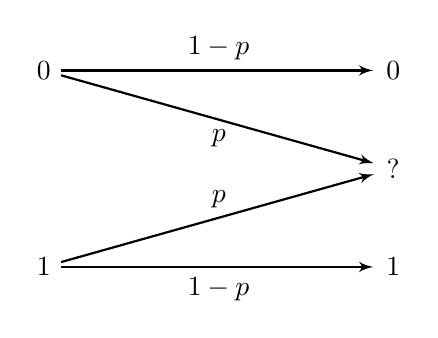
\begin{tikzpicture}[auto, thick, node distance=1 cm, ->,>=latex',shorten >=1pt]
	\node[] (0) {$0$};
	\node[right=4cm of 0] (0r) {$0$};	
	\node[below=0.75cm of 0r] (un) {$?$};
	\node[below=0.75cm of un] (1r) {$1$};
	\node[left=4cm of 1r] (1) {$1$};


	\path[every node]
		(0) edge node[above] {$1-p$} (0r)
		(1) edge node[below] {$1-p$} (1r)
		(0) edge node[below] {$p$} (un)
		(1) edge node[above] {$p$} (un);
\end{tikzpicture}
\caption{Binary Erasure Channel}
\label{fig:bec}
\end{figure}

The input symbol alphabet is $\mathcal{A}_x = \{0,1\}$ and the probability distribution of input symbols is
\begin{equation}
	p_x(a) = 
	\begin{cases}
		0 & \mbox{ with probability } q \\
		1 & \mbox{ with probability } 1- q \\
	\end{cases}
\end{equation}
The output symbol alphabet is $\mathcal{A}_y = \{0,?,1\}$. It is possible to compute the probability distribution of the output of the BEC with the total probability law by conditioning on the input symbol:
\begin{equation}
	p_y(b) = \sum_{a= 0}^1 p_x(a) p_{y|x}(b|a) = 
	\begin{cases}
		0, &\text{ wp } q(1-p)\\
		?, &\text{ wp } qp + (1-q)p = p\\
		1, &\text{ wp } (1-q)(1-p)\\
	\end{cases}
\end{equation}
Note that no transition is allowed from $0$ to $1$ and vice versa. Let $X$ be a random variable that describes the input symbols, i.e. with associated probability density function $p_x(a)$, and $Y$ the channel output random variable, with associated PDF $p_y(b)$. Then the capacity of the BEC is defined as
\begin{equation}
	C = \max_{p_x(a)} \, I(X;Y)
\end{equation}
In order to compute it is convenient to express the mutual information as
\begin{equation}
	I(X;Y) = H(Y) - H(Y|X)
\end{equation}
with $H(Y)$ the entropy of random variable $Y$ and $H(Y|X)$ the conditional entropy of $Y$ given $X$. Then
\begin{equation}
	H(Y) = \sum_{b\in\mathcal{A}_y} p_y(b) \log_2 \frac{1}{p_y(b)} = q(1-p)\log_2\frac{1}{q(1-p)} + p\log_2\frac{1}{p} + (1-q)(1-p)\log_2\frac{1}{(1-q)(1-p)}
\end{equation}
and
\begin{equation}
	H(Y|X) = \sum_{a\in\mathcal{A}_x, b\in\mathcal{A}_y} p_{y|x}(b|a)p_x(a)\log_2\frac{1}{p_{y|x}(b|a)p_x(a)} = \sum_{a=0}^1 p_x(a) \sum_{b\in\mathcal{A}_y}p_{y|x}(b|a)\log_2\frac{1}{p_{y|x}(b|a)}
\end{equation}
\begin{multline}\label{eq:hyx}
	H(Y|X) = q\left(p_{y|x}(0|0)\log_2\frac{1}{p_{y|x}(0|0)} + p_{y|x}(?|0)\log_2\frac{1}{p_{y|x}(?|0)}\right) + \\ (1-q)\left(p_{y|x}(1|1)\log_2\frac{1}{p_{y|x}(1|1)} + p_{y|x}(?|1)\log_2\frac{1}{p_{y|x}(?|1)}\right) = \\
	q\left((1-p)\log_2\frac{1}{1-p} + p\log_2\frac{1}{p} \right) + (1-q)\left((1-p)\log_2\frac{1}{1-p} + p\log_2\frac{1}{p}\right) = h(p)
\end{multline}
with 
\begin{equation}
	h(x) = (1-x)\log_2\frac{1}{1-x} + x\log_2\frac{1}{x}
\end{equation}
\begin{figure}[h]
\centering
\begin{tikzpicture}[
  declare function={
    func(\x)= and(\x>0, \x<1)*(-\x*log2{\x}-(1-\x)*log2{(1-\x)}) + and(\x==0, \x==1) * 0;
  },
]
\begin{axis}[
  axis x line=middle, axis y line=middle,
  ymin=0, ymax=1.1, ytick={0,1}, ylabel=$y$,
  xmin=0, xmax=1, xtick={0,0.5,1}, xlabel=$x$,
]
\addplot[black, domain=0:1, smooth]{func(x)};
\end{axis}
\end{tikzpicture} 
\caption{$h(x)$}
\label{fig:hx}
\end{figure}

Note that $p_{y|x}(0|1)\log_2\frac{1}{p_{y|x}(0|1)}$ and $p_{y|x}(1|0)\log_2\frac{1}{p_{y|x}(1|0)}$ were not included the summation in~\eqref{eq:hyx}. This is because $p_{y|x}(0|1) = p_{y|x}(1|0) = 0$, so both these terms are 0. Actually they are indeterminate forms $0\cdot\infty$, but the first factor of each product dominates and forces the result to 0.
Then let's compute the mutual information:
\begin{multline}
	I(X;Y) = H(Y) - H(Y|X) = q(1-p)\log_2\frac{1}{q(1-p)} + p\log_2\frac{1}{p} + (1-q)(1-p)\log_2\frac{1}{(1-q)(1-p)} \\ - (1-p)\log_2\frac{1}{1-p} - p\log_2\frac{1}{p}
\end{multline}
\begin{multline}
	I(X;Y) = (1-p)\left[q\log_2\frac{1}{q(1-p)} + (1-q)\log_2\frac{1}{(1-q)(1-p)} - \log_2\frac{1}{1-p} \right] = \\
		(1-p)\left[q\log_2\frac{1}{q} + q\log_2\frac{1}{1-p} + (1-q)\log_2\frac{1}{1-q} + (1-q)\log_2\frac{1}{1-p} - \log_2\frac{1}{1-p} \right]
\end{multline}
and finally
\begin{equation}
	I(X;Y) = (1-p)h(q)
\end{equation}
Note that the function $h(x)$ has a maximum equal to $1$ for $x=1/2$ as it can be seen in Fig.~\ref{fig:hx}. Therefore
\begin{equation}
	C = \max_{q} \; (1-p)h(q) = (1-p)
\end{equation}

\section*{Exercise 11 - Capacity of M-ary PAM channel with soft decoding}
In this exercise we will show some results on the mutual information and capacity that can be achieved on an M-ary PAM channel with soft decoding. 
Let the input symbols be $d_i \in \{0, \dots, M-1\}$ and the PAM symbols be $s_i \in \mathcal{S} = \{-M+1, -M+3, \dots, M-3, M-1\}$. The input symbols have probability distribution $p_x(a)$. The modulated symbols are sent on AWGN channel with Gaussian noise $w$ with variance
\begin{equation}
	\sigma_w^2 = \frac{E_s}{\Gamma}
\end{equation}
with $\Gamma$ the SNR and $E_s = \sum_{a \in \mathcal{S}} |a|^2 p_x(a)$ the energy of the constellation. In a AWGN channel transition PDFs have the form
\begin{equation}\label{eq:fy}
	f_{y|x}(b|a) = \frac{1}{\sqrt{2\pi}\sigma_w}e^{-\frac{(b-a)^2}{2\sigma_w^2}}
\end{equation}
Because the map from input to MAP symbols is invertible and because of the data processing inequality it is possible to compute the mutual information between input and output as the mutual information among random variables $x$ and $y$, describing the modulated symbols and the outputs.
Then the mutual information from \cite{erseghe} is
\begin{equation}
	I(X;Y) = H(y) - \frac{1}{2}\log_2(2\pi e\sigma_w^2)
\end{equation}
In particular the differential entropy of $y$ is
\begin{equation}\label{eq:hy}
	H(y) = \int f_y(b) \log_2\frac{1}{f_y(b)} db
\end{equation}
with
\begin{equation}
	f_y(b) = \sum_{a \in \mathcal{S}} f_{y|x}(b|a) p_x(a)
\end{equation}
The integral in~\eqref{eq:hy} can be computed only with numerical integration. A MATLAB script was written in order to evaluate it for different input distributions, modulation sizes $M$ and values of $\Gamma$. The script is in the attached listings. Notice that numerical stability problems may arise in performing the numerical integration. Since $\delta = 4.9407e-324$ is the lowest positive number which can be represented in MATLAB and that values below this threshold are approximated to $0$ by MATLAB, for high SNR $\Gamma$ (which corresponds to a small noise variance $\sigma_w^2$) the exponential term in~\eqref{eq:fy} tends rapidly to $\epsilon < \delta$ and therefore it is approximated to 0. Then the integrand of~\eqref{eq:hy} assumes an indeterminate value $0\cdot\infty$. However we remark that this is the product of a sum of exponentials and of a logarithm of the same sum, therefore the first term dominates the second on the limit and the actual value the integrand takes is 0. This was accounted for in the script by detecting \texttt{NaN} values in the integrand and replacing them with 0.

In Fig.~\ref{fig:info_uni} there is the plot of twice the mutual information that can be achieved with uniform input distribution. It does not reach the Shannon bound of $\log_2(1+\Gamma)$ but for SNR high enough it saturates to the maximum number of bits per second per hertz that the specific modulation can carry. 

In Fig.~\ref{fig:info_gauss} there is the plot of the mutual information obtained using an input with Gaussian distribution with a variance $\sigma_x^2 = E_s$ which maximizes the information rate for each SNR. Indeed, if the variance of the input distribution is kept fixed for all the SNRs it is not possible to reach capacity for in each SNR region: we need to design the input distribution in a different way for each SNR $\Gamma$, by keeping however the Gaussian shape. The Gaussian shape is imposed by computing
\begin{equation}
	p_x(a) = e^{-\frac{a^2}{2\sigma_{IN}^2}}
\end{equation}
and normalizing so that $\sum_{a \in \mathcal{S}} p_x(a) = 1$. The parameter $\sigma_{IN}$ controls the bell shape of the probability mass distribution.

\begin{figure}[t]
\centering
\setlength\fheight{0.5\textwidth}
\setlength\fwidth{0.75\textwidth}
% This file was created by matlab2tikz.
%
%The latest updates can be retrieved from
%  http://www.mathworks.com/matlabcentral/fileexchange/22022-matlab2tikz-matlab2tikz
%where you can also make suggestions and rate matlab2tikz.
%
\definecolor{mycolor1}{rgb}{0.01651,0.42660,0.87863}%
\definecolor{mycolor2}{rgb}{0.03434,0.59658,0.81985}%
\definecolor{mycolor3}{rgb}{0.14527,0.70976,0.66463}%
\definecolor{mycolor4}{rgb}{0.57086,0.74852,0.44939}%
\definecolor{mycolor5}{rgb}{0.72393,0.5579,0.45628}%
\definecolor{mycolor6}{rgb}{0.91887,0.72490,0.11324}%
\definecolor{mycolor7}{rgb}{0.12527,0.32424,0.83027}%
%
\begin{tikzpicture}

\begin{axis}[%
width=0.951\fwidth,
height=\fheight,
at={(0\fwidth,0\fheight)},
scale only axis,
xmin=0,
xmax=40,
xlabel={SNR $\Gamma$ [dB]},
xmajorgrids,
ymin=0,
ymax=14,
ylabel={$2I$ [bit/s/Hz]},
ymajorgrids,
axis background/.style={fill=white},
axis x line*=bottom,
axis y line*=left,
legend style={at={(0.03,0.97)},anchor=north west,legend cell align=left,align=left,draw=white!15!black}
]
\addplot [color=mycolor1,solid,line width=1.2pt,forget plot]
  table[row sep=crcr]{%
0	0.971875836891008\\
1	1.1255757443789\\
2	1.28429728132882\\
3	1.44132177726814\\
4	1.58870683330168\\
5	1.71838592743533\\
6	1.82376084762363\\
7	1.90136221319159\\
8	1.95195994879703\\
9	1.98032718480525\\
10	1.99351265597984\\
11	1.99836853797668\\
12	1.99970783240937\\
13	1.99996582350484\\
14	1.99999765791311\\
15	1.9999999180202\\
16	1.99999999876686\\
17	1.99999999999359\\
18	1.99999999999999\\
19	2\\
20	2\\
21	2\\
22	2.00000000000008\\
23	1.99999999999992\\
24	2.00000000000001\\
25	2\\
26	2\\
27	2\\
28	2\\
29	1.99999999999997\\
30	2.00000000288833\\
31	2.00000000000256\\
32	1.99999999999942\\
33	2.00000000000003\\
34	1.99999999999999\\
35	2.00000000003554\\
36	2.00000000000218\\
37	2.00000000000001\\
38	1.99999999999999\\
39	1.99999999999999\\
40	1.99999999999999\\
};
\addplot [color=mycolor1,line width=1.2pt,mark size=2.0pt,only marks,mark=o,mark options={solid},forget plot]
  table[row sep=crcr]{%
0	0.971875836891008\\
2	1.28429728132882\\
4	1.58870683330168\\
6	1.82376084762363\\
8	1.95195994879703\\
10	1.99351265597984\\
12	1.99970783240937\\
14	1.99999765791311\\
16	1.99999999876686\\
18	1.99999999999999\\
20	2\\
22	2.00000000000008\\
24	2.00000000000001\\
26	2\\
28	2\\
30	2.00000000288833\\
32	1.99999999999942\\
34	1.99999999999999\\
36	2.00000000000218\\
38	1.99999999999999\\
40	1.99999999999999\\
};
\addplot [color=mycolor1,solid,line width=1.2pt,mark size=2.0pt,mark=o,mark options={solid}]
  table[row sep=crcr]{%
0	0.971875836891008\\
};
\addlegendentry{M=2};

\addplot [color=mycolor2,solid,line width=1.2pt,forget plot]
  table[row sep=crcr]{%
0	0.989234438625861\\
1	1.15840373673096\\
2	1.3427068869805\\
3	1.54101587208338\\
4	1.75173138397283\\
5	1.97259215388577\\
6	2.20355529660951\\
7	2.44129727413542\\
8	2.68373573677848\\
9	2.92688217537811\\
10	3.16394318801\\
11	3.38516458385695\\
12	3.57940567902535\\
13	3.73705618970712\\
14	3.85302381169623\\
15	3.9285317101512\\
16	3.97079140237845\\
17	3.99039209502429\\
18	3.99759129565964\\
19	3.99957032516287\\
20	3.99994998447227\\
21	3.999996593559\\
22	3.99999988170082\\
23	3.99999999823932\\
24	3.99999999999099\\
25	3.99999999999999\\
26	4\\
27	4\\
28	3.99999999999988\\
29	4.00000000000198\\
30	4.00000000000007\\
31	4.00000000000001\\
32	4\\
33	4\\
34	3.99999999999998\\
35	4\\
36	3.99999999999994\\
37	4.00000000012603\\
38	3.9999999999988\\
39	4\\
40	4.00000000000002\\
};
\addplot [color=mycolor2,line width=1.2pt,mark size=2.0pt,only marks,mark=asterisk,mark options={solid},forget plot]
  table[row sep=crcr]{%
1	1.15840373673096\\
3	1.54101587208338\\
5	1.97259215388577\\
7	2.44129727413542\\
9	2.92688217537811\\
11	3.38516458385695\\
13	3.73705618970712\\
15	3.9285317101512\\
17	3.99039209502429\\
19	3.99957032516287\\
21	3.999996593559\\
23	3.99999999823932\\
25	3.99999999999999\\
27	4\\
29	4.00000000000198\\
31	4.00000000000001\\
33	4\\
35	4\\
37	4.00000000012603\\
39	4\\
40	4.00000000000002\\
};
\addplot [color=mycolor2,solid,line width=1.2pt,mark size=2.0pt,mark=asterisk,mark options={solid}]
  table[row sep=crcr]{%
1	1.15840373673096\\
};
\addlegendentry{M=4};

\addplot [color=mycolor3,solid,line width=1.2pt,forget plot]
  table[row sep=crcr]{%
0	0.990691205500404\\
1	1.16178583780303\\
2	1.34842920998677\\
3	1.55000399035013\\
4	1.76521076228336\\
5	1.99064655725971\\
6	2.23043380997702\\
7	2.47858045276801\\
8	2.73486210232677\\
9	2.99849465314343\\
10	3.26857235195456\\
11	3.54421459045778\\
12	3.82456815406646\\
13	4.10871224815384\\
14	4.39528022832985\\
15	4.68143288930338\\
16	4.96127882905534\\
17	5.22499071348098\\
18	5.46007816460856\\
19	5.65470283584332\\
20	5.80146179703933\\
21	5.90000210816481\\
22	5.95729721630836\\
23	5.98516084167029\\
24	5.99601523528946\\
25	5.99922525097086\\
26	5.99989952559402\\
27	5.99999216256497\\
28	5.99999967726035\\
29	5.99999999405062\\
30	5.99999999996015\\
31	5.99999999999992\\
32	6.00000000000001\\
33	6\\
34	5.99999999999998\\
35	6.00000000000004\\
36	5.99999999999997\\
37	6\\
38	5.99999999999953\\
39	6.00000000000011\\
40	6.00000000046429\\
};
\addplot [color=mycolor3,line width=1.2pt,mark size=2.0pt,only marks,mark=x,mark options={solid},forget plot]
  table[row sep=crcr]{%
0	0.990691205500404\\
2	1.34842920998677\\
4	1.76521076228336\\
6	2.23043380997702\\
8	2.73486210232677\\
10	3.26857235195456\\
12	3.82456815406646\\
14	4.39528022832985\\
16	4.96127882905534\\
18	5.46007816460856\\
20	5.80146179703933\\
22	5.95729721630836\\
24	5.99601523528946\\
26	5.99989952559402\\
28	5.99999967726035\\
30	5.99999999996015\\
32	6.00000000000001\\
34	5.99999999999998\\
36	5.99999999999997\\
38	5.99999999999953\\
40	6.00000000046429\\
};
\addplot [color=mycolor3,solid,line width=1.2pt,mark size=2.0pt,mark=x,mark options={solid}]
  table[row sep=crcr]{%
0	0.990691205500404\\
};
\addlegendentry{M=8};

\addplot [color=mycolor4,solid,line width=1.2pt,forget plot]
  table[row sep=crcr]{%
0	0.9908601124796\\
1	1.16247155337467\\
2	1.34962898161056\\
3	1.55188026275746\\
4	1.76799828338336\\
5	1.99381630050754\\
6	2.23565797818477\\
7	2.48581392922009\\
8	2.74433905316268\\
9	3.01060941926089\\
10	3.28382230660841\\
11	3.56320173043889\\
12	3.8480435078334\\
13	4.13771348241822\\
14	4.43163884223986\\
15	4.72929915730997\\
16	5.03021722107803\\
17	5.33394864680704\\
18	5.64006431426131\\
19	5.94807955548703\\
20	6.25711640111142\\
21	6.56486526768312\\
22	6.86582689286191\\
23	7.15013404663123\\
24	7.40469176655757\\
25	7.61668328937306\\
26	7.77772900200843\\
27	7.8868629641333\\
28	7.95104715139954\\
29	7.98270724965265\\
30	7.9952599248893\\
31	7.99905434611928\\
32	7.99987333720775\\
33	7.99998971034696\\
34	7.99999955414453\\
35	7.99999999123916\\
36	7.99999999993647\\
37	7.99999999999986\\
38	8\\
39	8.00000000000056\\
40	7.99999999999994\\
};
\addplot [color=mycolor4,line width=1.2pt,mark size=1.4pt,only marks,mark=square,mark options={solid},forget plot]
  table[row sep=crcr]{%
1	1.16247155337467\\
3	1.55188026275746\\
5	1.99381630050754\\
7	2.48581392922009\\
9	3.01060941926089\\
11	3.56320173043889\\
13	4.13771348241822\\
15	4.72929915730997\\
17	5.33394864680704\\
19	5.94807955548703\\
21	6.56486526768312\\
23	7.15013404663123\\
25	7.61668328937306\\
27	7.8868629641333\\
29	7.98270724965265\\
31	7.99905434611928\\
33	7.99998971034696\\
35	7.99999999123916\\
37	7.99999999999986\\
39	8.00000000000056\\
40	7.99999999999994\\
};
\addplot [color=mycolor4,solid,line width=1.2pt,mark size=1.4pt,mark=square,mark options={solid}]
  table[row sep=crcr]{%
1	1.16247155337467\\
};
\addlegendentry{M=16};

\addplot [color=mycolor5,solid,line width=1.2pt,forget plot]
  table[row sep=crcr]{%
0	0.990832625971208\\
1	1.1626246509154\\
2	1.34991538362636\\
3	1.55232946415346\\
4	1.76866442327927\\
5	1.99438422673316\\
6	2.23684890525917\\
7	2.48751408391272\\
8	2.74656652404849\\
9	3.0134380738193\\
10	3.28734928355309\\
11	3.56753857883933\\
12	3.85331659774905\\
13	4.14406714737897\\
14	4.43923984108601\\
15	4.73834276899973\\
16	5.04093588275463\\
17	5.3466250269452\\
18	5.65505651776388\\
19	5.96591216325229\\
20	6.27890456039762\\
21	6.59377130452077\\
22	6.91025367193796\\
23	7.22819619025422\\
24	7.54731208762553\\
25	7.86735726186661\\
26	8.18769451380006\\
27	8.50627701902558\\
28	8.81780777244928\\
29	9.11241487716187\\
30	9.37671735213307\\
31	9.59741869396302\\
32	9.76565200872286\\
33	9.88013886486017\\
34	9.94782467969967\\
35	9.9814297782641\\
36	9.9948617041711\\
37	9.99896283127155\\
38	9.99985898808911\\
39	9.99998832940456\\
40	9.99999948217369\\
};
\addplot [color=mycolor5,line width=1.2pt,mark size=3pt,only marks,mark=diamond,mark options={solid},forget plot]
  table[row sep=crcr]{%
0	0.990832625971208\\
2	1.34991538362636\\
4	1.76866442327927\\
6	2.23684890525917\\
8	2.74656652404849\\
10	3.28734928355309\\
12	3.85331659774905\\
14	4.43923984108601\\
16	5.04093588275463\\
18	5.65505651776388\\
20	6.27890456039762\\
22	6.91025367193796\\
24	7.54731208762553\\
26	8.18769451380006\\
28	8.81780777244928\\
30	9.37671735213307\\
32	9.76565200872286\\
34	9.94782467969967\\
36	9.9948617041711\\
38	9.99985898808911\\
40	9.99999948217369\\
};
\addplot [color=mycolor5,solid,line width=1.2pt,mark size=3pt,mark=diamond,mark options={solid}]
  table[row sep=crcr]{%
0	0.990832625971208\\
};
\addlegendentry{M=32};

\addplot [color=mycolor6,solid,line width=1.2pt,forget plot]
  table[row sep=crcr]{%
0	0.990766013036129\\
1	1.1626531589372\\
2	1.34998526538749\\
3	1.55244051133358\\
4	1.76882910913564\\
5	1.99437835409706\\
6	2.23711031182587\\
7	2.48792795285935\\
8	2.74711451236876\\
9	3.01413354969178\\
10	3.28821464534693\\
11	3.56859974963058\\
12	3.85460242919167\\
13	4.145609790564\\
14	4.44107529983145\\
15	4.7405115672999\\
16	5.0434838758334\\
17	5.34960440531541\\
18	5.65852707630037\\
19	5.96994294318975\\
20	6.28357607372541\\
21	6.5991798573985\\
22	6.91653368915408\\
23	7.23543997805977\\
24	7.55572143098916\\
25	7.87721856041399\\
26	8.19978767283426\\
27	8.5232989690088\\
28	8.84762762017165\\
29	9.1726676973849\\
30	9.49830716272332\\
31	9.82438698740058\\
32	10.1503950209778\\
33	10.4744325902364\\
34	10.7913377519916\\
35	11.0912757546988\\
36	11.3607431143951\\
37	11.586188472036\\
38	11.7584525332425\\
39	11.8760335459657\\
40	11.9458070648569\\
};
\addplot [color=mycolor6,line width=1.2pt,mark size=1.3pt,only marks,mark=triangle,mark options={solid},forget plot]
  table[row sep=crcr]{%
0	0.990766013036129\\
2	1.34998526538749\\
4	1.76882910913564\\
6	2.23711031182587\\
8	2.74711451236876\\
10	3.28821464534693\\
12	3.85460242919167\\
14	4.44107529983145\\
16	5.0434838758334\\
18	5.65852707630037\\
20	6.28357607372541\\
22	6.91653368915408\\
24	7.55572143098916\\
26	8.19978767283426\\
28	8.84762762017165\\
30	9.49830716272332\\
32	10.1503950209778\\
34	10.7913377519916\\
36	11.3607431143951\\
38	11.7584525332425\\
40	11.9458070648569\\
};
\addplot [color=mycolor6,solid,line width=1.2pt,mark size=1.3pt,mark=triangle,mark options={solid}]
  table[row sep=crcr]{%
0	0.990766013036129\\
};
\addlegendentry{M=64};

\addplot [color=mycolor7,solid,line width=1.2pt,forget plot]
  table[row sep=crcr]{%
0	1\\
1	1.17563663469239\\
2	1.37010466975099\\
3	1.58268235491156\\
4	1.81224619130063\\
5	2.0573732086068\\
6	2.31645617962626\\
7	2.58781437356203\\
8	2.86978721917029\\
9	3.16080442391302\\
10	3.4594316186373\\
11	3.76439436704286\\
12	4.07458523490543\\
13	4.38905896736305\\
14	4.70702026272884\\
15	5.02780767335052\\
16	5.3508761542486\\
17	5.67577990180488\\
18	6.00215644400198\\
19	6.32971245944191\\
20	6.65821148275179\\
21	6.98746345895592\\
22	7.31731600193655\\
23	7.64764716249041\\
24	7.97835949780125\\
25	8.30937524121281\\
26	8.64063238901739\\
27	8.97208154332096\\
28	9.30368337320288\\
29	9.63540657832163\\
30	9.96722625883599\\
31	10.2991226126573\\
32	10.6310798956186\\
33	10.963085592331\\
34	11.2951297555622\\
35	11.627204480216\\
36	11.959303484698\\
37	12.2914217778744\\
38	12.6235553942094\\
39	12.9557011831739\\
40	13.2878566418405\\
};
\addplot [color=mycolor7,line width=1.2pt,mark size=1.3pt,only marks,mark=triangle,mark options={solid,rotate=180},forget plot]
  table[row sep=crcr]{%
0	1\\
2	1.37010466975099\\
4	1.81224619130063\\
6	2.31645617962626\\
8	2.86978721917029\\
10	3.4594316186373\\
12	4.07458523490543\\
14	4.70702026272884\\
16	5.3508761542486\\
18	6.00215644400198\\
20	6.65821148275179\\
22	7.31731600193655\\
24	7.97835949780125\\
26	8.64063238901739\\
28	9.30368337320288\\
30	9.96722625883599\\
32	10.6310798956186\\
34	11.2951297555622\\
36	11.959303484698\\
38	12.6235553942094\\
40	13.2878566418405\\
};
\addplot [color=mycolor7,solid,line width=1.2pt,mark size=1.3pt,mark=triangle,mark options={solid,rotate=180}]
  table[row sep=crcr]{%
0	1\\
};
\addlegendentry{Shannon bound};

\end{axis}
\end{tikzpicture}%
\caption{Information rate for M-ary PAM, soft decoding, with uniform input probabilities}
\label{fig:info_uni}
\end{figure}
\begin{figure}[t]
\centering
\setlength\fheight{0.5\textwidth}
\setlength\fwidth{0.75\textwidth}
% This file was created by matlab2tikz.
%
%The latest updates can be retrieved from
%  http://www.mathworks.com/matlabcentral/fileexchange/22022-matlab2tikz-matlab2tikz
%where you can also make suggestions and rate matlab2tikz.
%
\definecolor{mycolor1}{rgb}{0.01651,0.42660,0.87863}%
\definecolor{mycolor2}{rgb}{0.03434,0.59658,0.81985}%
\definecolor{mycolor3}{rgb}{0.14527,0.70976,0.66463}%
\definecolor{mycolor4}{rgb}{0.57086,0.74852,0.44939}%
\definecolor{mycolor5}{rgb}{0.72393,0.5579,0.45628}%
\definecolor{mycolor6}{rgb}{0.91887,0.72490,0.11324}%
\definecolor{mycolor7}{rgb}{0.12527,0.32424,0.83027}%
%
\begin{tikzpicture}

\begin{axis}[%
width=0.951\fwidth,
height=\fheight,
at={(0\fwidth,0\fheight)},
scale only axis,
xmin=0,
xmax=40,
xlabel={SNR $\Gamma$ [dB]},
xmajorgrids,
ymin=0,
ymax=14,
ylabel={$2C$ [bit/s/Hz]},
ymajorgrids,
axis background/.style={fill=white},
axis x line*=bottom,
axis y line*=left,
legend style={at={(0.03,0.97)},anchor=north west,legend cell align=left,align=left,draw=white!15!black}
]
\addplot [color=mycolor1,solid,line width=1.2pt,forget plot]
  table[row sep=crcr]{%
0	0.971888308097055\\
1	1.12557627553976\\
2	1.28429729118252\\
3	1.44132177733225\\
4	1.58870683330218\\
5	1.71838816749885\\
6	1.82376090917411\\
7	1.90136221385157\\
8	1.95195994876569\\
9	1.98032718519313\\
10	1.99351265598005\\
11	1.99836853795366\\
12	1.99970783240798\\
13	1.99996582350908\\
14	1.99999765791283\\
15	1.99999991802027\\
16	1.99999999876686\\
17	1.99999999999359\\
18	1.99999999999999\\
19	2\\
20	2\\
21	2\\
22	1.9999999999997\\
23	2.00000000000019\\
24	1.99999999999994\\
25	2.00000000000001\\
26	2\\
27	2\\
28	1.99999999999999\\
29	2\\
30	2\\
31	1.99999999999962\\
32	2.00000000000072\\
33	1.99999999999959\\
34	2.00000000000006\\
35	2.00000000000002\\
36	2.00000000000001\\
37	1.99999999999998\\
38	2.00000000000001\\
39	1.99999997730462\\
40	1.99999999826715\\
};
\addplot [color=mycolor1,line width=1.2pt,mark size=2.0pt,only marks,mark=o,mark options={solid},forget plot]
  table[row sep=crcr]{%
0	0.971888308097055\\
2	1.28429729118252\\
4	1.58870683330218\\
6	1.82376090917411\\
8	1.95195994876569\\
10	1.99351265598005\\
12	1.99970783240798\\
14	1.99999765791283\\
16	1.99999999876686\\
18	1.99999999999999\\
20	2\\
22	1.9999999999997\\
24	1.99999999999994\\
26	2\\
28	1.99999999999999\\
30	2\\
32	2.00000000000072\\
34	2.00000000000006\\
36	2.00000000000001\\
38	2.00000000000001\\
40	1.99999999826715\\
};
\addplot [color=mycolor1,solid,line width=1.2pt,mark size=2.0pt,mark=o,mark options={solid}]
  table[row sep=crcr]{%
0	0.971888308097055\\
};
\addlegendentry{M=2};

\addplot [color=mycolor2,solid,line width=1.2pt,forget plot]
  table[row sep=crcr]{%
0	0.999345551548677\\
1	1.17454529456039\\
2	1.36825419160005\\
3	1.57932295999415\\
4	1.80550402892047\\
5	2.04280774136323\\
6	2.28471143545748\\
7	2.52754800431933\\
8	2.78298270250817\\
9	3.02991079208923\\
10	3.25649883984145\\
11	3.45240990721973\\
12	3.62906502845971\\
13	3.76541354777161\\
14	3.86672784063135\\
15	3.93366865349079\\
16	3.97218136509966\\
17	3.9906363859352\\
18	3.99761520707933\\
19	3.99954772733602\\
20	3.9999158871508\\
21	3.99996069451522\\
22	3.99996382200811\\
23	3.99996393144418\\
24	3.99996393306655\\
25	3.9999639330748\\
26	3.99996393307481\\
27	3.99996393307473\\
28	3.99996393307481\\
29	3.99996393307468\\
30	3.99996393307491\\
31	3.99996393307479\\
32	3.99996393307482\\
33	3.99996393307482\\
34	3.99996393307482\\
35	3.99996393307483\\
36	3.99996393307478\\
37	3.99996393307478\\
38	3.99996393307466\\
39	3.99996393307508\\
40	3.99996393307454\\
};
\addplot [color=mycolor2,line width=1.2pt,mark size=2.0pt,only marks,mark=asterisk,mark options={solid},forget plot]
  table[row sep=crcr]{%
1	1.17454529456039\\
3	1.57932295999415\\
5	2.04280774136323\\
7	2.52754800431933\\
9	3.02991079208923\\
11	3.45240990721973\\
13	3.76541354777161\\
15	3.93366865349079\\
17	3.9906363859352\\
19	3.99954772733602\\
21	3.99996069451522\\
23	3.99996393144418\\
25	3.9999639330748\\
27	3.99996393307473\\
29	3.99996393307468\\
31	3.99996393307479\\
33	3.99996393307482\\
35	3.99996393307483\\
37	3.99996393307478\\
39	3.99996393307508\\
40	3.99996393307454\\
};
\addplot [color=mycolor2,solid,line width=1.2pt,mark size=2.0pt,mark=asterisk,mark options={solid}]
  table[row sep=crcr]{%
1	1.17454529456039\\
};
\addlegendentry{M=4};

\addplot [color=mycolor3,solid,line width=1.2pt,forget plot]
  table[row sep=crcr]{%
0	0.999391805678989\\
1	1.1746683787104\\
2	1.36863208140618\\
3	1.58053791140833\\
4	1.80924687241234\\
5	2.05332970276561\\
6	2.31118145164513\\
7	2.5811291812529\\
8	2.86151532634135\\
9	3.15071166833724\\
10	3.44690085692982\\
11	3.74729062093844\\
12	4.04662548832161\\
13	4.33579858360336\\
14	4.60210124836562\\
15	4.87662896825513\\
16	5.13913264222959\\
17	5.36396461912406\\
18	5.55292845926277\\
19	5.71171495243168\\
20	5.83009239273558\\
21	5.91108768496036\\
22	5.96060062904523\\
23	5.9858107340639\\
24	5.9960913443873\\
25	5.99920727974027\\
26	5.99985702270874\\
27	5.99994536985341\\
28	5.99995245218093\\
29	5.9999527466222\\
30	5.99995275218003\\
31	5.99995275221634\\
32	5.99995275221666\\
33	5.99995275221605\\
34	5.99995275221634\\
35	5.99995275221597\\
36	5.99995275221633\\
37	5.99995275221621\\
38	5.99995275221623\\
39	5.99995275221625\\
40	5.99995275221628\\
};
\addplot [color=mycolor3,line width=1.2pt,mark size=2.0pt,only marks,mark=x,mark options={solid},forget plot]
  table[row sep=crcr]{%
0	0.999391805678989\\
2	1.36863208140618\\
4	1.80924687241234\\
6	2.31118145164513\\
8	2.86151532634135\\
10	3.44690085692982\\
12	4.04662548832161\\
14	4.60210124836562\\
16	5.13913264222959\\
18	5.55292845926277\\
20	5.83009239273558\\
22	5.96060062904523\\
24	5.9960913443873\\
26	5.99985702270874\\
28	5.99995245218093\\
30	5.99995275218003\\
32	5.99995275221666\\
34	5.99995275221634\\
36	5.99995275221633\\
38	5.99995275221623\\
40	5.99995275221628\\
};
\addplot [color=mycolor3,solid,line width=1.2pt,mark size=2.0pt,mark=x,mark options={solid}]
  table[row sep=crcr]{%
0	0.999391805678989\\
};
\addlegendentry{M=8};

\addplot [color=mycolor4,solid,line width=1.2pt,forget plot]
  table[row sep=crcr]{%
0	0.999408682444212\\
1	1.17469745280493\\
2	1.36868095755175\\
3	1.5806181058597\\
4	1.80937523001774\\
5	2.05353006246288\\
6	2.31148668624484\\
7	2.58158433058098\\
8	2.86218804490596\\
9	3.15175554843269\\
10	3.44887991843473\\
11	3.7523112815447\\
12	4.06096226360329\\
13	4.37390204429842\\
14	4.69034154413577\\
15	5.00959117838038\\
16	5.33085781201407\\
17	5.65249112854234\\
18	5.97034984586825\\
19	6.2760471881737\\
20	6.55696204783422\\
21	6.81936365907557\\
22	7.0954838849052\\
23	7.3321954518299\\
24	7.52196636321313\\
25	7.69144867160002\\
26	7.81520043143389\\
27	7.90192422009003\\
28	7.95553692632077\\
29	7.9836198888852\\
30	7.99537128062514\\
31	7.99904157958184\\
32	7.99982940018522\\
33	7.99994016121595\\
34	7.99994941035314\\
35	7.99994981502477\\
36	7.99994982303188\\
37	7.99994982334478\\
38	7.99994982309716\\
39	7.99994982308889\\
40	7.99994982308926\\
};
\addplot [color=mycolor4,line width=1.2pt,mark size=1.4pt,only marks,mark=square,mark options={solid},forget plot]
  table[row sep=crcr]{%
1	1.17469745280493\\
3	1.5806181058597\\
5	2.05353006246288\\
7	2.58158433058098\\
9	3.15175554843269\\
11	3.7523112815447\\
13	4.37390204429842\\
15	5.00959117838038\\
17	5.65249112854234\\
19	6.2760471881737\\
21	6.81936365907557\\
23	7.3321954518299\\
25	7.69144867160002\\
27	7.90192422009003\\
29	7.9836198888852\\
31	7.99904157958184\\
33	7.99994016121595\\
35	7.99994981502477\\
37	7.99994982334478\\
39	7.99994982308889\\
40	7.99994982308926\\
};
\addplot [color=mycolor4,solid,line width=1.2pt,mark size=1.4pt,mark=square,mark options={solid}]
  table[row sep=crcr]{%
1	1.17469745280493\\
};
\addlegendentry{M=16};

\addplot [color=mycolor5,solid,line width=1.2pt,forget plot]
  table[row sep=crcr]{%
0	0.999413237424212\\
1	1.17470516478925\\
2	1.36869365356741\\
3	1.58063844895953\\
4	1.80940696056953\\
5	2.0535782369021\\
6	2.31155789862524\\
7	2.5816869163286\\
8	2.86233228189339\\
9	3.15195388541598\\
10	3.44914727556183\\
11	3.7526654861449\\
12	4.06142471684085\\
13	4.37449883703404\\
14	4.69110703609899\\
15	5.01059796707123\\
16	5.33243273997342\\
17	5.65616827687631\\
18	5.98144189053654\\
19	6.30795745574927\\
20	6.63547212917995\\
21	6.96376610309879\\
22	7.29247151624272\\
23	7.62036436500294\\
24	7.94372580636136\\
25	8.25448400069983\\
26	8.54011628739805\\
27	8.79427780671357\\
28	9.07604266419012\\
29	9.31792344772567\\
30	9.50882254130661\\
31	9.68171432907968\\
32	9.80783277714561\\
33	9.89735334410267\\
34	9.9530252820617\\
35	9.98249793070846\\
36	9.99499413574643\\
37	9.9989533574332\\
38	9.9998150976262\\
39	9.99993813317178\\
40	9.99994860397205\\
};
\addplot [color=mycolor5,line width=1.2pt,mark size=3pt,only marks,mark=diamond,mark options={solid},forget plot]
  table[row sep=crcr]{%
0	0.999413237424212\\
2	1.36869365356741\\
4	1.80940696056953\\
6	2.31155789862524\\
8	2.86233228189339\\
10	3.44914727556183\\
12	4.06142471684085\\
14	4.69110703609899\\
16	5.33243273997342\\
18	5.98144189053654\\
20	6.63547212917995\\
22	7.29247151624272\\
24	7.94372580636136\\
26	8.54011628739805\\
28	9.07604266419012\\
30	9.50882254130661\\
32	9.80783277714561\\
34	9.9530252820617\\
36	9.99499413574643\\
38	9.9998150976262\\
40	9.99994860397205\\
};
\addplot [color=mycolor5,solid,line width=1.2pt,mark size=3pt,mark=diamond,mark options={solid}]
  table[row sep=crcr]{%
0	0.999413237424212\\
};
\addlegendentry{M=32};

\addplot [color=mycolor6,solid,line width=1.2pt,forget plot]
  table[row sep=crcr]{%
0	0.999414393596782\\
1	1.17470711543369\\
2	1.36869685102552\\
3	1.58064354689848\\
4	1.8094148687617\\
5	2.05359017292287\\
6	2.31157543182063\\
7	2.58171200239735\\
8	2.86236728950979\\
9	3.1520016186607\\
10	3.44921099727874\\
11	3.75274894786571\\
12	4.06153220111252\\
13	4.37463521830173\\
14	4.69127786733383\\
15	5.01080960155983\\
16	5.33269250198496\\
17	5.6564847029382\\
18	5.98182507718073\\
19	6.30841961011753\\
20	6.63602958759096\\
21	6.96446155357863\\
22	7.29355889474622\\
23	7.62319481718543\\
24	7.95326663860121\\
25	8.28369094981941\\
26	8.61439871663727\\
27	8.94531421896591\\
28	9.27620003069936\\
29	9.60597549863665\\
30	9.93109154764579\\
31	10.243635240484\\
32	10.5311616530548\\
33	10.7803828355937\\
34	11.0649010228553\\
35	11.3095074830408\\
36	11.5029246652065\\
37	11.6757893556982\\
38	11.8032921568636\\
39	11.8944975276846\\
40	11.9514311401169\\
};
\addplot [color=mycolor6,line width=1.2pt,mark size=1.3pt,only marks,mark=triangle,mark options={solid},forget plot]
  table[row sep=crcr]{%
0	0.999414393596782\\
2	1.36869685102552\\
4	1.8094148687617\\
6	2.31157543182063\\
8	2.86236728950979\\
10	3.44921099727874\\
12	4.06153220111252\\
14	4.69127786733383\\
16	5.33269250198496\\
18	5.98182507718073\\
20	6.63602958759096\\
22	7.29355889474622\\
24	7.95326663860121\\
26	8.61439871663727\\
28	9.27620003069936\\
30	9.93109154764579\\
32	10.5311616530548\\
34	11.0649010228553\\
36	11.5029246652065\\
38	11.8032921568636\\
40	11.9514311401169\\
};
\addplot [color=mycolor6,solid,line width=1.2pt,mark size=1.3pt,mark=triangle,mark options={solid}]
  table[row sep=crcr]{%
0	0.999414393596782\\
};
\addlegendentry{M=64};

\addplot [color=mycolor7,solid,line width=1.2pt,forget plot]
  table[row sep=crcr]{%
0	1\\
1	1.17563663469239\\
2	1.37010466975099\\
3	1.58268235491156\\
4	1.81224619130063\\
5	2.0573732086068\\
6	2.31645617962626\\
7	2.58781437356203\\
8	2.86978721917029\\
9	3.16080442391302\\
10	3.4594316186373\\
11	3.76439436704286\\
12	4.07458523490543\\
13	4.38905896736305\\
14	4.70702026272884\\
15	5.02780767335052\\
16	5.3508761542486\\
17	5.67577990180488\\
18	6.00215644400198\\
19	6.32971245944191\\
20	6.65821148275179\\
21	6.98746345895592\\
22	7.31731600193655\\
23	7.64764716249041\\
24	7.97835949780125\\
25	8.30937524121281\\
26	8.64063238901739\\
27	8.97208154332096\\
28	9.30368337320288\\
29	9.63540657832163\\
30	9.96722625883599\\
31	10.2991226126573\\
32	10.6310798956186\\
33	10.963085592331\\
34	11.2951297555622\\
35	11.627204480216\\
36	11.959303484698\\
37	12.2914217778744\\
38	12.6235553942094\\
39	12.9557011831739\\
40	13.2878566418405\\
};
\addplot [color=mycolor7,line width=1.2pt,mark size=1.3pt,only marks,mark=triangle,mark options={solid,rotate=180},forget plot]
  table[row sep=crcr]{%
0	1\\
2	1.37010466975099\\
4	1.81224619130063\\
6	2.31645617962626\\
8	2.86978721917029\\
10	3.4594316186373\\
12	4.07458523490543\\
14	4.70702026272884\\
16	5.3508761542486\\
18	6.00215644400198\\
20	6.65821148275179\\
22	7.31731600193655\\
24	7.97835949780125\\
26	8.64063238901739\\
28	9.30368337320288\\
30	9.96722625883599\\
32	10.6310798956186\\
34	11.2951297555622\\
36	11.959303484698\\
38	12.6235553942094\\
40	13.2878566418405\\
};
\addplot [color=mycolor7,solid,line width=1.2pt,mark size=1.3pt,mark=triangle,mark options={solid,rotate=180}]
  table[row sep=crcr]{%
0	1\\
};
\addlegendentry{Shannon bound};

\end{axis}
\end{tikzpicture}%
\caption{Capacity for M-ary PAM, soft decoding, with Gaussian input probabilities}
\label{fig:info_gauss}
\end{figure}

\begin{figure*}[t]
\centering
\subfloat[Information rate for 32-ary PAM, soft decoding, with Gaussian input probabilities, different $\sigma_{IN}$ values]{\setlength\fheight{0.45\textwidth}
\setlength\fwidth{0.4\textwidth}
% This file was created by matlab2tikz.
%
%The latest updates can be retrieved from
%  http://www.mathworks.com/matlabcentral/fileexchange/22022-matlab2tikz-matlab2tikz
%where you can also make suggestions and rate matlab2tikz.
%
\definecolor{mycolor1}{rgb}{0.01651,0.42660,0.87863}%
\definecolor{mycolor2}{rgb}{0.57086,0.74852,0.44939}%
\definecolor{mycolor3}{rgb}{0.14527,0.70976,0.66463}%
\definecolor{mycolor4}{rgb}{0.12527,0.01424,0.9027}%
%
\begin{tikzpicture}

\begin{axis}[%
width=0.951\fwidth,
height=\fheight,
at={(0\fwidth,0\fheight)},
scale only axis,
xmin=22,
xmax=38,
xlabel={SNR $\Gamma$ [dB]},
xmajorgrids,
ymin=6,
ymax=11,
ylabel={$2I$ [bit/s/Hz]},
ymajorgrids,
axis background/.style={fill=white},
axis x line*=bottom,
axis y line*=left,
legend style={at={(1-0.03,1-0.97)},anchor=south east,legend cell align=left,align=left,draw=white!15!black}
]

\addplot [color=mycolor4,solid,line width=1.2pt,forget plot]
  table[row sep=crcr]{%
0 0.990832625971208\\
1 1.1626246509154\\
2 1.34991538362636\\
3 1.55232946415346\\
4 1.76866442327927\\
5 1.99438422673316\\
6 2.23684890525917\\
7 2.48751408391272\\
8 2.74656652404849\\
9 3.0134380738193\\
10  3.28734928355309\\
11  3.56753857883933\\
12  3.85331659774905\\
13  4.14406714737897\\
14  4.43923984108601\\
15  4.73834276899973\\
16  5.04093588275463\\
17  5.3466250269452\\
18  5.65505651776388\\
19  5.96591216325229\\
20  6.27890456039762\\
21  6.59377130452077\\
22  6.91025367193796\\
23  7.22819619025422\\
24  7.54731208762553\\
25  7.86735726186661\\
26  8.18769451380006\\
27  8.50627701902558\\
28  8.81780777244928\\
29  9.11241487716187\\
30  9.37671735213307\\
31  9.59741869396302\\
32  9.76565200872286\\
33  9.88013886486017\\
34  9.94782467969967\\
35  9.9814297782641\\
36  9.9948617041711\\
37  9.99896283127155\\
38  9.99985898808911\\
39  9.99998832940456\\
40  9.99999948217369\\
};
\addplot [color=mycolor4,line width=1.2pt,mark size=1pt,only marks,mark=diamond,mark options={solid},forget plot]
  table[row sep=crcr]{%
0 0.990832625971208\\
2 1.34991538362636\\
4 1.76866442327927\\
6 2.23684890525917\\
8 2.74656652404849\\
10  3.28734928355309\\
12  3.85331659774905\\
14  4.43923984108601\\
16  5.04093588275463\\
18  5.65505651776388\\
20  6.27890456039762\\
22  6.91025367193796\\
24  7.54731208762553\\
26  8.18769451380006\\
28  8.81780777244928\\
30  9.37671735213307\\
32  9.76565200872286\\
34  9.94782467969967\\
36  9.9948617041711\\
38  9.99985898808911\\
40  9.99999948217369\\
};
\addplot [color=mycolor4,solid,line width=1.2pt,mark size=1pt,mark=diamond,mark options={solid}]
  table[row sep=crcr]{%
0 0.990832625971208\\
};
\addlegendentry{Uniform distribution};

\addplot [color=mycolor1,solid,line width=1.2pt,forget plot]
  table[row sep=crcr]{%
0	0.999413237424212\\
1	1.17470516478925\\
2	1.36869365356741\\
3	1.58063844895953\\
4	1.80940696056953\\
5	2.0535782369021\\
6	2.31155789862524\\
7	2.5816869163286\\
8	2.86233228189339\\
9	3.15195388541598\\
10	3.44914727556183\\
11	3.7526654861449\\
12	4.06142471684085\\
13	4.37449883703404\\
14	4.69110703609899\\
15	5.01059796707123\\
16	5.33243273997342\\
17	5.65616827687631\\
18	5.98144189053654\\
19	6.30795745574927\\
20	6.63547212917995\\
21	6.96376610309879\\
22	7.29247151624272\\
23	7.62036436500294\\
24	7.94372580636136\\
25	8.25448400069983\\
26	8.54011628739805\\
27	8.78641069281901\\
28	8.9818847411391\\
29	9.12174034272503\\
30	9.20972040339597\\
31	9.25689977537135\\
32	9.27765038048656\\
33	9.28478525749247\\
34	9.28659228512173\\
35	9.28690539684257\\
36	9.28693928430935\\
37	9.28694132931659\\
38	9.28694138906613\\
39	9.28694138987441\\
40	9.28694138976643\\
};
\addplot [color=mycolor1,line width=1.2pt,mark size=1pt,only marks,mark=o,mark options={solid},forget plot]
  table[row sep=crcr]{%
1	1.17470516478925\\
3	1.58063844895953\\
5	2.0535782369021\\
7	2.5816869163286\\
9	3.15195388541598\\
11	3.7526654861449\\
13	4.37449883703404\\
15	5.01059796707123\\
17	5.65616827687631\\
19	6.30795745574927\\
21	6.96376610309879\\
23	7.62036436500294\\
25	8.25448400069983\\
27	8.78641069281901\\
29	9.12174034272503\\
31	9.25689977537135\\
33	9.28478525749247\\
35	9.28690539684257\\
37	9.28694132931659\\
39	9.28694138987441\\
40	9.28694138976643\\
};
\addplot [color=mycolor1,solid,line width=1.2pt,mark size=1pt,mark=o,mark options={solid}]
  table[row sep=crcr]{%
1	1.17470516478925\\
};
\addlegendentry{$\sigma{}_\text{IN}\text{=12.8}$};

\addplot [color=mycolor2,solid,line width=1.2pt,forget plot]
  table[row sep=crcr]{%
0	0.994291182286695\\
1	1.16626467442649\\
2	1.35545295346972\\
3	1.56085984864018\\
4	1.78122461816132\\
5	2.01515624222313\\
6	2.2612387605889\\
7	2.51810094290944\\
8	2.78445758887059\\
9	3.05913157863596\\
10	3.34106296314098\\
11	3.62930930587561\\
12	3.92304041786907\\
13	4.2215298413661\\
14	4.52414475835222\\
15	4.8303354432872\\
16	5.13962495923747\\
17	5.45159948840265\\
18	5.7658994784751\\
19	6.08221163766682\\
20	6.40026170723164\\
21	6.71980784562295\\
22	7.04063430342284\\
23	7.3625438030491\\
24	7.6853310775977\\
25	8.00861735052441\\
26	8.33116119994222\\
27	8.64926185967274\\
28	8.95494799796887\\
29	9.23588912196973\\
30	9.47810911079102\\
31	9.67032542325069\\
32	9.80783277714561\\
33	9.89432429041979\\
34	9.94069900403226\\
35	9.96109261768589\\
36	9.96810355627258\\
37	9.96987885180955\\
38	9.9701864123934\\
39	9.97021968582476\\
40	9.97022169277204\\
};
\addplot [color=mycolor2,line width=1.2pt,mark size=1.5pt,only marks,mark=diamond,mark options={solid},forget plot]
  table[row sep=crcr]{%
0	0.994291182286695\\
2	1.35545295346972\\
4	1.78122461816132\\
6	2.2612387605889\\
8	2.78445758887059\\
10	3.34106296314098\\
12	3.92304041786907\\
14	4.52414475835222\\
16	5.13962495923747\\
18	5.7658994784751\\
20	6.40026170723164\\
22	7.04063430342284\\
24	7.6853310775977\\
26	8.33116119994222\\
28	8.95494799796887\\
30	9.47810911079102\\
32	9.80783277714561\\
34	9.94069900403226\\
36	9.96810355627258\\
38	9.9701864123934\\
40	9.97022169277204\\
};
\addplot [color=mycolor2,solid,line width=1.2pt,mark size=1.5pt,mark=diamond,mark options={solid}]
  table[row sep=crcr]{%
0	0.994291182286695\\
};
\addlegendentry{$\sigma{}_\text{IN}\text{=32}$};

\addplot [color=mycolor3,solid,line width=1.2pt,forget plot]
  table[row sep=crcr]{%
0	0.992395271814619\\
1	1.16302674790626\\
2	1.35018418682848\\
3	1.5527046868447\\
4	1.76921858501786\\
5	1.99831558958783\\
6	2.2386550204168\\
7	2.4890134791893\\
8	2.74829241419891\\
9	3.01551009088342\\
10	3.28979037826383\\
11	3.57035183201307\\
12	3.85649762963689\\
13	4.14760639616935\\
14	4.44312388740511\\
15	4.74255547276717\\
16	5.0454593476579\\
17	5.35144039460417\\
18	5.6601446049465\\
19	5.97125396161754\\
20	6.28448166567835\\
21	6.5995675364478\\
22	6.91627337522753\\
23	7.23437764969425\\
24	7.55366480584984\\
25	7.87386505102535\\
26	8.19432569188509\\
27	8.51294866089701\\
28	8.82433998306976\\
29	9.11852077562002\\
30	9.38205981044063\\
31	9.6017102899483\\
32	9.76874914912808\\
33	9.88209188244261\\
34	9.94885910974825\\
35	9.98185946441811\\
36	9.99497615984944\\
37	9.9989533574332\\
38	9.9998150976262\\
39	9.99993813317178\\
40	9.99994860397205\\
};
\addplot [color=mycolor3,line width=1.2pt,mark size=1pt,only marks,mark=x,mark options={solid},forget plot]
  table[row sep=crcr]{%
0	0.992395271814619\\
2	1.35018418682848\\
4	1.76921858501786\\
6	2.2386550204168\\
8	2.74829241419891\\
10	3.28979037826383\\
12	3.85649762963689\\
14	4.44312388740511\\
16	5.0454593476579\\
18	5.6601446049465\\
20	6.28448166567835\\
22	6.91627337522753\\
24	7.55366480584984\\
26	8.19432569188509\\
28	8.82433998306976\\
30	9.38205981044063\\
32	9.76874914912808\\
34	9.94885910974825\\
36	9.99497615984944\\
38	9.9998150976262\\
40	9.99994860397205\\
};
\addplot [color=mycolor3,solid,line width=1.2pt,mark size=1pt,mark=x,mark options={solid}]
  table[row sep=crcr]{%
0	0.992395271814619\\
};
\addlegendentry{$\sigma{}_\text{IN}\text{=160}$};


\end{axis}
\end{tikzpicture}%
\label{fig:info_gauss_32}
}
\subfloat[Gaussian input probabilities, different $\sigma_{IN}$ values]{\setlength\fheight{0.45\textwidth}
\setlength\fwidth{0.4\textwidth}
% This file was created by matlab2tikz.
%
%The latest updates can be retrieved from
%  http://www.mathworks.com/matlabcentral/fileexchange/22022-matlab2tikz-matlab2tikz
%where you can also make suggestions and rate matlab2tikz.
%
\definecolor{mycolor1}{rgb}{0.01651,0.42660,0.87863}%
\definecolor{mycolor2}{rgb}{0.57086,0.74852,0.44939}%
\definecolor{mycolor3}{rgb}{0.14527,0.70976,0.66463}%
%
\begin{tikzpicture}

\begin{axis}[%
width=0.951\fwidth,
height=\fheight,
at={(0\fwidth,0\fheight)},
scale only axis,
xmin=-35,
xmax=35,
xlabel={a},
xmajorgrids,
ymin=0,
ymax=0.07,
ylabel={$\text{p}_\text{x}\text{(a)}$},
ymajorgrids,
axis background/.style={fill=white},
axis x line*=bottom,
axis y line*=left,
legend style={at={(0.03,0.97)},anchor=north west,legend cell align=left,align=left,draw=white!15!black}
]
\addplot[ycomb,color=mycolor1,solid,line width=1.2pt,mark size=1.0pt,mark=o,mark options={solid}] plot table[row sep=crcr] {%
-31	0.00336082517387937\\
-29	0.00484718182370738\\
-27	0.00682228420901484\\
-25	0.0093706002617749\\
-23	0.0125603610454977\\
-21	0.0164298630029326\\
-19	0.0209731116309685\\
-17	0.0261269613035598\\
-15	0.0317623072861028\\
-13	0.0376818565046449\\
-11	0.0436264271395267\\
-9	0.0492906006304176\\
-7	0.054347013153925\\
-5	0.0584769022997213\\
-3	0.0614030782823173\\
-1	0.0629206262520093\\
1	0.0629206262520093\\
3	0.0614030782823173\\
5	0.0584769022997213\\
7	0.054347013153925\\
9	0.0492906006304176\\
11	0.0436264271395267\\
13	0.0376818565046449\\
15	0.0317623072861028\\
17	0.0261269613035598\\
19	0.0209731116309685\\
21	0.0164298630029326\\
23	0.0125603610454977\\
25	0.0093706002617749\\
27	0.00682228420901484\\
29	0.00484718182370738\\
31	0.00336082517387937\\
};
\addlegendentry{$\sigma{}_\text{IN}\text{=12.8}$};

\addplot[ycomb,color=mycolor2,solid,line width=1.2pt,mark size=2.0pt,mark=diamond,mark options={solid}] plot table[row sep=crcr] {%
-31	0.022841738358871\\
-29	0.0242201090883352\\
-27	0.0255815334652609\\
-25	0.0269141451975336\\
-23	0.0282057819939844\\
-21	0.0294441645328965\\
-19	0.030617086705166\\
-17	0.0317126131266011\\
-15	0.0327192795279402\\
-13	0.0336262913678001\\
-11	0.0344237158874592\\
-9	0.0351026628467804\\
-7	0.0356554493519082\\
-5	0.0360757445060343\\
-3	0.0363586900769901\\
-1	0.0365009939664387\\
1	0.0365009939664387\\
3	0.0363586900769901\\
5	0.0360757445060343\\
7	0.0356554493519082\\
9	0.0351026628467804\\
11	0.0344237158874592\\
13	0.0336262913678001\\
15	0.0327192795279402\\
17	0.0317126131266011\\
19	0.030617086705166\\
21	0.0294441645328965\\
23	0.0282057819939844\\
25	0.0269141451975336\\
27	0.0255815334652609\\
29	0.0242201090883352\\
31	0.022841738358871\\
};
\addlegendentry{$\sigma{}_\text{IN}\text{=32}$};

\addplot[ycomb,color=mycolor3,solid,line width=1.2pt,mark size=2.0pt,mark=x,mark options={solid}] plot table[row sep=crcr] {%
-31	0.0308733185115891\\
-29	0.0309457627142383\\
-27	0.0310135306643477\\
-25	0.0310765909224022\\
-23	0.0311349141913594\\
-21	0.0311884733393337\\
-19	0.0312372434206301\\
-17	0.031281201695108\\
-15	0.0313203276458516\\
-13	0.031354602995129\\
-11	0.0313840117186221\\
-9	0.0314085400579122\\
-7	0.0314281765312071\\
-5	0.0314429119422983\\
-3	0.0314527393877386\\
-1	0.0314576542622325\\
1	0.0314576542622325\\
3	0.0314527393877386\\
5	0.0314429119422983\\
7	0.0314281765312071\\
9	0.0314085400579122\\
11	0.0313840117186221\\
13	0.031354602995129\\
15	0.0313203276458516\\
17	0.031281201695108\\
19	0.0312372434206301\\
21	0.0311884733393337\\
23	0.0311349141913594\\
25	0.0310765909224022\\
27	0.0310135306643477\\
29	0.0309457627142383\\
31	0.0308733185115891\\
};
\addlegendentry{$\sigma{}_\text{IN}\text{=160}$};

\end{axis}
\end{tikzpicture}%
\label{fig:pxa}
}
\hfil
\subfloat[$\sigma_{IN}$ that maximizes the information rate for each SNR $\Gamma$]{\setlength\fheight{0.45\textwidth}
\setlength\fwidth{0.4\textwidth}
% This file was created by matlab2tikz.
%
%The latest updates can be retrieved from
%  http://www.mathworks.com/matlabcentral/fileexchange/22022-matlab2tikz-matlab2tikz
%where you can also make suggestions and rate matlab2tikz.
%
\definecolor{mycolor1}{rgb}{0.04981,0.45857,0.86406}%
%
\begin{tikzpicture}

\begin{axis}[%
width=0.951\fwidth,
height=\fheight,
at={(0\fwidth,0\fheight)},
scale only axis,
xmin=20,
xmax=36,
xlabel={SNR $\Gamma$ [dB]},
xmajorgrids,
ymin=0,
ymax=140,
ylabel={$\sigma{}_\text{IN}$},
ymajorgrids,
axis background/.style={fill=white},
axis x line*=bottom,
axis y line*=left,
legend style={at={(0.03,0.97)},anchor=north west,legend cell align=left,align=left,draw=white!15!black}
]
\addplot [color=mycolor1,solid,line width=1.2pt,forget plot]
  table[row sep=crcr]{%
20	9\\
21	10\\
22	10\\
23	11\\
24	12\\
25	13\\
26	14\\
27	15\\
28	17\\
29	19\\
30	22\\
31	25\\
32	30\\
33	38\\
34	52\\
35	76\\
36	127\\
};
\addplot [color=mycolor1,line width=1.2pt,mark size=2.0pt,only marks,mark=o,mark options={solid},forget plot]
  table[row sep=crcr]{%
20	9\\
21	10\\
22	10\\
22	10\\
23	11\\
24	12\\
25	13\\
26	14\\
26	14\\
27	15\\
28	17\\
29	19\\
30	22\\
30	22\\
31	25\\
32	30\\
33	38\\
34	52\\
34	52\\
35	76\\
36	127\\
};
\addplot [color=mycolor1,solid,line width=1.2pt,mark size=2.0pt,mark=o,mark options={solid}]
  table[row sep=crcr]{%
20	9\\
};
\addlegendentry{$\sigma{}_\text{IN}$};

\end{axis}
\end{tikzpicture}%
\label{fig:sigmax}
}
\end{figure*}

\clearpage

The need for a different design for each SNR $\Gamma$ can be seen in Fig.~\ref{fig:info_gauss_32}, where the mutual information with Gaussian inputs with different values for the parameter $\sigma_{IN} \in [0.4, 1, 5]M$ is compared, for $M=32$. We can notice that for SNR $\Gamma < 28$~dB the highest mutual information is achieved for $\sigma_{IN} = 12.8$, but this input distribution does not manage to reach the saturation value for SNR $\Gamma > 35$~dB. This is reached instead by $\sigma_{IN} = 160$. For intermediate values of SNR the value that dominates is $\sigma_{IN} = 32$. The reason behind this behavior is that a distribution with a very high weight for the symbols at the center of the constellation and a low weight (close to 0) for symbols which are close to $\pm(M-1)$ resembles a constellation with a number of symbols $M' < M$ and it is not able to achieve the mutual information of $\log_2(M)$ bit per symbol. However the Gaussian shape improves the performances for lower SNRs, when the mutual information is not in saturation. In order to get to the saturation value of $\log_2(M)$ bit per symbol (or twice this value in the plot) the input distribution should be designed in order to use with equal probability all the symbols, i.e. it should be uniform. This is why for $M = 32$ the saturation value is reached for very high $\sigma_{IN}$ values, ideally for $\sigma_{IN} \rightarrow \infty$, i.e. for a true uniform distribution. The different shapes of the input distribution can be seen in~\ref{fig:pxa}.
In Fig.~\ref{fig:sigmax} we plot the $\sigma_{IN}$ value that maximizes the mutual information for each $\Gamma \in [20, 36]$ and $M=32$. It can be seen that as the SNR grows $\sigma_{IN}$ tends to $\infty$.

Notice that the higher the value of $M$ the more this behavior can be observed. Indeed for small constellations there is no room of improvement by changing the parameter $\sigma_{IN}$, and thus the shape of the input distribution, up to the degenerate case of $M=2$ where each symmetric distribution (as the Gaussian one) is also uniform.

\begin{thebibliography}{10}

\bibitem{erseghe} Tomaso Erseghe, \emph{Channel Coding}, A graduate course blueprint, 2015

\end{thebibliography}

\end{document}
